\documentclass[12pt,letterpaper,reqno]{article}

% \usepackage{mathtools}
\usepackage{epsfig}
\usepackage{amsmath}
\usepackage{amssymb}
\usepackage{amsthm}
\usepackage{indentfirst}
\usepackage{xspace}
\usepackage{multirow}
\usepackage{hyperref}
\usepackage{xcolor}
\usepackage{verbatim}
\usepackage[letterpaper,margin=1in,headheight=15pt]{geometry}
\usepackage{mathpazo}
\usepackage{tikz-cd}
\usepackage{booktabs}
\usepackage{framed}
\usepackage{float}
\usepackage{thmtools}
\usepackage{dashrule}
\usepackage[missing=]{gitinfo2}
\usepackage{fancyhdr}
\usepackage{slashed}
\usepackage{soul}
\usepackage[makeroom]{cancel}



\definecolor{darkblue}{rgb}{0.1,0.1,0.7}
\definecolor{darkred}{rgb}{0.5,0.1,0.1}
\definecolor{purple}{RGB}{128,0,128}
\definecolor{darkgreen}{rgb}{0.0,0.42,0.06}
\hypersetup{colorlinks=true,urlcolor=darkred,linkcolor=darkblue,citecolor=darkred}
\definecolor{shadecolor}{rgb}{0.85,0.85,0.85}

% Bibliography formatting
\usepackage[bibstyle=authoryear-comp,labeldate=false,defernumbers=true,maxnames=20,uniquename=init,dashed=false,backend=biber,sorting=none]{biblatex}

\DeclareNameAlias{sortname}{first-last}

\DeclareFieldFormat{url}{\url{#1}}
\DeclareFieldFormat[article]{pages}{#1}
\DeclareFieldFormat[inproceedings]{pages}{\lowercase{pp.}#1}
\DeclareFieldFormat[incollection]{pages}{\lowercase{pp.}#1}
\DeclareFieldFormat[article]{volume}{\textbf{#1}}
\DeclareFieldFormat[article]{number}{(#1)}
\DeclareFieldFormat[article]{title}{\MakeCapital{#1}}
\DeclareFieldFormat[inproceedings]{title}{#1}
\DeclareFieldFormat{shorthandwidth}{#1}

% Don't use "In:" in bibliography. Omit urls from journal articles.
\DeclareBibliographyDriver{article}{%
  \usebibmacro{bibindex}%
  \usebibmacro{begentry}%
  \usebibmacro{author/editor}%
  \setunit{\labelnamepunct}\newblock
  \MakeSentenceCase{\usebibmacro{title}}%
  \newunit
  \printlist{language}%
  \newunit\newblock
  \usebibmacro{byauthor}%
  \newunit\newblock
  \usebibmacro{byeditor+others}%
  \newunit\newblock
  \printfield{version}%
  \newunit\newblock
%  \usebibmacro{in:}%
  \usebibmacro{journal+issuetitle}%
  \newunit\newblock
  \printfield{note}%
  \setunit{\bibpagespunct}%
  \printfield{pages}
  \newunit\newblock
  \usebibmacro{eprint}
  \newunit\newblock
  \printfield{addendum}%
  \newunit\newblock
  \usebibmacro{pageref}%
  \usebibmacro{finentry}}

% Remove dot between volume and number in journal articles.
\renewbibmacro*{journal+issuetitle}{%
  \usebibmacro{journal}%
  \setunit*{\addspace}%
  \iffieldundef{series}
    {}
    {\newunit
     \printfield{series}%
     \setunit{\addspace}}%
  \printfield{volume}%
%  \setunit*{\adddot}%
  \printfield{number}%
  \setunit{\addcomma\space}%
  \printfield{eid}%
  \setunit{\addspace}%
  \usebibmacro{issue+date}%
  \newunit\newblock
  \usebibmacro{issue}%
  \newunit}


% Bibliography categories
\def\makebibcategory#1#2{\DeclareBibliographyCategory{#1}\defbibheading{#1}{\section*{#2}}}
\makebibcategory{books}{Books}
\makebibcategory{papers}{Refereed research papers}
\makebibcategory{chapters}{Book chapters}
\makebibcategory{conferences}{Papers in conference proceedings}
\makebibcategory{techreports}{Unpublished working papers}
\makebibcategory{bookreviews}{Book reviews}
\makebibcategory{editorials}{Editorials}
\makebibcategory{phd}{PhD thesis}
\makebibcategory{subpapers}{Submitted papers}
\makebibcategory{curpapers}{Current projects}

\setlength{\bibitemsep}{2.65pt}
\setlength{\bibhang}{.8cm}
\renewcommand{\bibfont}{\small}

\renewcommand*{\bibitem}{\addtocounter{papers}{1}\item \mbox{}\hskip-0.85cm\hbox to 0.85cm{\hfill\arabic{papers}.~~}}
\defbibenvironment{bibliography}
{\list{}
  {\setlength{\leftmargin}{\bibhang}%
   \setlength{\itemsep}{\bibitemsep}%
   \setlength{\parsep}{\bibparsep}}}
{\endlist}
{\bibitem}

\newenvironment{publications}{\section{\LARGE Publications}\label{papersstart}\vspace*{0.2cm}\small
\titlespacing{\section}{0pt}{1.5ex}{1ex}\itemsep=0.00cm
}{\label{papersend}\addtocounter{sumpapers}{-1}\refstepcounter{sumpapers}\label{sumpapers}}

\def\printbib#1{\printbibliography[category=#1,heading=#1]\lastref{sumpapers}}

% Counters for keeping track of papers
\newcounter{papers}\setcounter{papers}{0}
\newcounter{sumpapers}\setcounter{sumpapers}{0}
\def\lastref#1{\addtocounter{#1}{\value{papers}}\setcounter{papers}{0}}

% theorem environments
\declaretheoremstyle[spaceabove=0.25cm,spacebelow=0.25cm,notefont=\normalfont\bfseries, notebraces={(}{)}]{theorem}
\declaretheoremstyle[spaceabove=0.25cm,spacebelow=0.25cm,bodyfont=\normalfont,notefont=\normalfont\bfseries, notebraces={(}{)}]{noital}
\declaretheoremstyle[spaceabove=0.25cm,spacebelow=0.25cm,bodyfont=\normalfont\color{darkgreen},notefont=\normalfont\bfseries, notebraces={(}{)}]{green}
\declaretheoremstyle[spaceabove=0.25cm,spacebelow=0.25cm,bodyfont=\normalfont\color{purple},notefont=\normalfont\bfseries, notebraces={(}{)}]{sbrown}
\declaretheoremstyle[spaceabove=0.25cm,spacebelow=0.25cm,bodyfont=\normalfont,notefont=\normalfont\bfseries,qed=$\qedsymbol$,notebraces={(}{)}]{proofstyle}

\declaretheorem[name=Theorem,numberwithin=section,style=theorem]{thm}
\declaretheorem[name=Fact,numberwithin=section,style=theorem]{fact}
\declaretheorem[name=Proposition,sibling=thm,style=theorem]{prop}
\declaretheorem[name=Corollary,sibling=thm,style=theorem]{cor}
\declaretheorem[name=Lemma,sibling=thm,style=theorem]{lem}
\declaretheorem[name=Definition,sibling=thm,style=noital]{defn}
\declaretheorem[name=Example,sibling=thm,style=noital]{example}
\declaretheorem[name=Exercise,numberwithin=section,style=green]{exercise}
\declaretheorem[name=Solution,numberwithin=section,style=sbrown]{solution}
\declaretheorem[name=Proof,style=proofstyle,numbered=no]{pf}

\numberwithin{equation}{section}


% macros for convenience
\newcommand{\tops}{\texorpdfstring}

\newcommand{\nid}{\noindent}

\newcommand{\fa}{{\mathfrak a}}
\newcommand{\fp}{{\mathfrak p}}
\newcommand{\fk}{{\mathfrak k}}
\newcommand{\fg}{{\mathfrak g}}
\newcommand{\fh}{{\mathfrak h}}
\newcommand{\fn}{{\mathfrak n}}
\newcommand{\fq}{{\mathfrak q}}
\newcommand{\fm}{{\mathfrak m}}
\newcommand{\fr}{{\mathfrak r}}
\newcommand{\fu}{{\mathfrak u}}
\newcommand{\fG}{{\mathfrak G}}
\newcommand{\fso}{{\mathfrak {so}}}

\newcommand{\cC}{\ensuremath{\mathcal C}}
\newcommand{\cG}{\ensuremath{\mathcal G}}
\newcommand{\cB}{\ensuremath{\mathcal B}}
\newcommand{\cL}{\ensuremath{\mathcal L}}
\newcommand{\cS}{\ensuremath{\mathcal S}}
\newcommand{\cF}{\ensuremath{\mathcal F}}
\newcommand{\cK}{\ensuremath{\mathcal K}}
\newcommand{\cZ}{\ensuremath{\mathcal Z}}
\newcommand{\cM}{\ensuremath{\mathcal M}}
\newcommand{\cN}{\ensuremath{\mathcal N}}
\newcommand{\cO}{\ensuremath{\mathcal O}}
\newcommand{\cH}{\ensuremath{\mathcal H}}
\newcommand{\cX}{\ensuremath{\mathcal X}}
\newcommand{\cY}{\ensuremath{\mathcal Y}}
\newcommand{\cA}{\ensuremath{\mathcal A}}
\newcommand{\cI}{\ensuremath{\mathcal I}}

\newcommand{\R}{\ensuremath{\mathbb R}}
\newcommand{\C}{\ensuremath{\mathbb C}}
\newcommand{\PP}{\ensuremath{\mathbb P}}
\newcommand{\Z}{\ensuremath{\mathbb Z}}
\newcommand{\Q}{\ensuremath{\mathbb Q}}
\newcommand{\A}{\ensuremath{\mathbb A}}
\newcommand{\bbH}{\ensuremath{\mathbb H}}
\newcommand{\bbI}{\ensuremath{\mathbb I}}
\newcommand{\bS}{\ensuremath{\mathbb S}}

\newcommand{\half}{\ensuremath{\frac{1}{2}}}
\newcommand{\qtr}{\ensuremath{\frac{1}{4}}}
\newcommand{\bq}{{\mathbf q}}
\newcommand{\N}{{\mathcal N}}
\newcommand{\F}{{\mathcal F}}
\newcommand{\HH}{{\mathcal H}}
\newcommand{\LL}{{\mathcal L}}
\newcommand{\RR}{{\mathcal R}}
\newcommand{\V}{{\mathcal V}}
\newcommand{\dirac}{\!\!\not\!\partial}
\newcommand{\Dirac}{\!\!\not\!\!D}
\newcommand{\cE}{{\mathcal E}}
\newcommand{\vs}{\not\!v}
\newcommand{\kahler}{K\"ahler\xspace}
\newcommand{\kq}{/\!\!/}
\newcommand{\kql}[1]{/\!\!/\!\!_#1\,}
\newcommand{\hk}{hyperk\"ahler\xspace}
\newcommand{\Hk}{Hyperk\"ahler\xspace}
\newcommand{\hkq}{/\!\!/\!\!/\!\!/}
\newcommand{\hkql}[1]{/\!\!/\!\!/\!\!/\!\!_#1\,}
\newcommand{\del}{\ensuremath{\partial}}
\newcommand{\delbar}{\ensuremath{\overline{\partial}}}
\newcommand{\I}{{\mathrm i}}
\newcommand{\J}{{\mathrm j}}
\newcommand{\K}{{\mathrm k}}
\newcommand{\e}{{\mathrm e}}
\newcommand\bid{{\mathbf 1}}
\newcommand{\de}{\mathrm{d}}
\newcommand{\ab}{\mathrm{ab}}
\newcommand{\vol}{\mathrm{vol}}
\renewcommand{\sf}{\mathrm{sf}}
\newcommand{\inst}{\mathrm{inst}}
\newcommand{\eff}{\mathrm{eff}}
\newcommand{\rmtop}{\mathrm{top}}
\newcommand{\rmbot}{\mathrm{bot}}
\newcommand{\dR}{\mathrm{dR}}
\newcommand{\closed}{\mathrm{closed}}
\newcommand{\exact}{\mathrm{exact}}

\newcommand{\abs}[1]{\lvert#1\rvert}
\newcommand{\norm}[1]{\lVert#1\rVert}
\newcommand{\IP}[1]{\langle#1\rangle}
\newcommand{\DIP}[1]{\langle\!\langle#1\rangle\!\rangle}
\newcommand{\dwrt}[1]{\frac{\partial}{\partial#1}}
\newcommand{\eps}{\epsilon}
\newcommand{\simarrow}{\xrightarrow\sim}

\newcommand{\tlambda}{\widetilde\lambda}

\newcommand{\mmaref}[1]{}

\newcommand{\ti}[1]{\textit{#1}}
\newcommand{\tb}[1]{\textbf{#1}}

\DeclareMathOperator{\sgn}{sgn}
\DeclareMathOperator{\dvol}{dvol}
\DeclareMathOperator{\ad}{ad}
\DeclareMathOperator{\im}{Im}
\DeclareMathOperator{\re}{Re}
\DeclareMathOperator{\Tr}{Tr}
\DeclareMathOperator{\End}{End}
\DeclareMathOperator{\Hom}{Hom}
\DeclareMathOperator{\Aut}{Aut}
\DeclareMathOperator{\Sym}{Sym}
\DeclareMathOperator{\Lie}{Lie}
\DeclareMathOperator{\diag}{diag}
\DeclareMathOperator{\Bun}{Bun}
\DeclareMathOperator{\Vect}{Vect}
\DeclareMathOperator{\Span}{Span}
\DeclareMathOperator{\grad}{grad}
\DeclareMathOperator{\rank}{rank}
\DeclareMathOperator{\ind}{ind}
\DeclareMathOperator{\coker}{coker}
\DeclareMathOperator{\Jac}{Jac}
\DeclareMathOperator{\Hol}{Hol}
\DeclareMathOperator{\gr}{gr}
\DeclareMathOperator{\Pin}{Pin}
\DeclareMathOperator{\Spin}{Spin}
\DeclareMathOperator{\SO}{SO}
\DeclareMathOperator{\SU}{SU}
\DeclareMathOperator{\U}{U}
\DeclareMathOperator{\Cliff}{Cliff}
\DeclareMathOperator{\vertices}{vertices}
\DeclareMathOperator{\edges}{edges}
\DeclareMathOperator{\Obs}{Obs}
\DeclareMathOperator{\Ber}{Ber}
\DeclareMathOperator{\Pf}{Pf}
\DeclareMathOperator{\Euler}{Euler}
\DeclareMathOperator{\Hess}{Hess}
\DeclareMathOperator{\Map}{Map}

\newcommand{\insfig}[2]{

\medskip
\noindent
\begin{minipage}{\linewidth}
\makebox[\linewidth]{\includegraphics[keepaspectratio=true,scale=#2]{figures/#1-crop.pdf}}
\end{minipage}
\noindent}


% \newcommand{\insfig}[2]{\begin{figure}[htbp] \centering \includegraphics[scale=#2]{figures/#1-crop.pdf} \label{fig:#1} \end{figure}}
% syntax: \insfig{name}{0.5}{caption}

\newcommand{\fixme}[1]{{\color{orange}{[#1]}}}
\newcommand{\currentposition}{{\color{blue} \noindent\makebox[\linewidth]{\hdashrule{\paperwidth}{1pt}{3mm}}}}

% \mathtoolsset{showonlyrefs}

\bibliography{qft-geometry}

\begin{document}

\pagestyle{fancy}
\lhead{{\tiny \color{gray} \tt \gitAuthorIsoDate}}
\chead{\tiny \ti{Applications of QFT to Geometry, \tb{preliminary} and \tb{incomplete} draft}}
\rhead{{\tiny \color{gray} \tt \gitAbbrevHash}}
\renewcommand{\headrulewidth}{0.5pt}


\begin{center}
\tb{Applications of QFT to Geometry} \\
Andrew Neitzke \\
\tb{Preliminary} and \tb{incomplete} draft
\end{center}

{These are the notes for a Fall 2017
course at UT Austin, \ti{in progress}.
They are extremely incomplete, unreliable, full
of mistakes and omissions.
The latest PDF can always be found
at
\begin{center}
\small \url{http://ma.utexas.edu/users/neitzke/teaching/392C-qft-geometry/qft-geometry.pdf}
\end{center}
Please send corrections/improvements to
\begin{center}
\small \tt\href{mailto:neitzke@math.utexas.edu}{neitzke@math.utexas.edu}
\end{center}
or as pull requests to the source repository hosted at
\begin{center}
\small \url{http://github.com/neitzke/qft-geometry}
\end{center}
I thank Arun Debray, Behzat Ergun, Robbie Rosati 
and Ivan Tulli for very helpful
suggestions and corrections.

You can join a Slack channel for the course (needs {\tt {@math.utexas.edu}} address)
at
\begin{center}
\small \url{https://join.slack.com/t/qft-geometry/signup} 
\end{center}
}

% \tableofcontents
% \renewcommand{\listtheoremname}{Quick reference}
% \listoftheorems[onlynamed]

% \newpage

%\setcounter{page}{1}


\section{Introductory motivation}

\subsection{Linear equations}
Suppose we are interested in studying
the topology of smooth manifolds $X$.
One powerful tool for this purpose is to
introduce an ingredient which at first seems alien to the
problem: namely we fix a Riemannian metric $g$ on $X$.
This allows us to define the \ti{form Laplacian} \eqref{eq:form-laplacian}
and consider the space of \ti{harmonic forms}
\begin{equation}
  \cH_k(X) = \{ \omega \in \Omega^k(X) \vert \Delta \omega = 0 \}.
\end{equation}

The equation
\begin{equation} \label{eq:laplace}
\Delta \omega = 0
\end{equation}
is a \ti{linear} equation over $\R$.
Thus $\cH_k(X)$ is a \ti{vector space}.
If $X$ is compact, then $\cH_k(X)$ is moreover finite-dimensional (a consequence of
the fact that $\Delta$ is an \ti{elliptic} operator). Thus we can define
positive integers by
\begin{equation}
  b_k(X) = \dim_\R \cH_k(X).
\end{equation}
There is a remarkable fact about these integers:
\begin{fact} \label{fact:betti-numbers-are-topological} The integers $b_k$ do not depend on the choice of Riemannian metric or smooth
structure on $X$; instead they are invariants of the underlying topological manifold
(the \ti{Betti numbers}).
\end{fact}

\begin{exercise} Work out explicitly the spaces $\cH^k(X)$ and
Betti numbers $b_k(X)$ for some of the following: $X = S^1, T^2, S^2$.
(In each case choose a convenient Riemannian metric; of course the $b_k$
are independent of which metric you choose, though the $\cH_k(X)$
naively are not.)
\end{exercise}
\begin{solution}
From \eqref{eq:form-laplacian} we have the definition of actual adjoint $d^*:\Omega^k(X)\to\Omega^{k-1}(X)$ as
\begin{equation}
  \langle d^*\alpha,\beta\rangle=\langle\alpha,d\beta\rangle
\end{equation}
which defines the Laplace operator $\Delta=dd^*+d^*d:\Omega^k(X)\to\Omega^k(X)$ on the Riemannian manifold $X$
\begin{enumerate}
\item First we note that the manifold $X=S^1$ can only have $\Omega^0(X)$ and $\Omega^1(X)$ (because higher forms vanish). Next, we put a flat metric $g_{00}=1$ on the circle $S^1$.  We consider $\alpha\in\Omega^1(X)$ and $\beta\in\Omega^0(X)$ then in the chart $\theta:S^1\to\mathbb{R}$, $\alpha = f(\theta)d\theta$ and $\beta=h(\theta)$.  Now $d^*$ can be evaluated as follows
  \begin{equation}
    \begin{split}
       \langle d^*\alpha,\beta\rangle&=\langle\alpha,d\beta\rangle\\   
       &=\int f(\theta)\partial_\theta h(\theta)\sqrt{g}d\theta\\
       &=\int\frac{1}{\sqrt{g}}(-\partial_\theta)(\sqrt{g} f(\theta))h(\theta)\sqrt{g}d\theta
    \end{split}
  \end{equation}
Now the Laplacian $\Delta=dd^*+d^*d$ acting on $\alpha\in\Omega^0(S^1)$ is essentially $d^*d\alpha$ (because $d^*$ annhiliates $\alpha$).  Therefore in the chart $\theta$, $\Delta=\partial^2_\theta$.  Now $\mathcal{H}_0(X)=\{\omega\in\Omega^0(X)|\partial^2_\theta\omega(\theta)=0\}$.  The solution $\omega(\theta)=a\theta+b$ resulting in $b_0(S^1)=1$ (?).

Next, for $\alpha\in\Omega^1(S^1)$, the Laplacian operator $\Delta = dd^*$.  In the chart $\theta$, we have $\alpha = f(\theta)d\theta$ and $\Delta\alpha=\partial_\theta^2f(\theta)d\theta$.  Similar to last time, $f(\theta)$ is harmonic and $b_1(S^1)=1$
\item Let $x,y:T^2\to\mathbb{R}^2$ be the chart for two-torous.  We put a flat metric $g_{ij}=\delta_{ij}$ where $i,j\in x,y$.  Repeating the procedure from the $S^1$ case, we have
  \begin{equation}
    d^*\equiv \frac{1}{\sqrt{g}}\partial_i(\sqrt{g}g^{ij}\partial_j)
  \end{equation}
Now for $T^2$ manifold, only the forms in $\Omega^k(T^2)$ where $k\in (0,2)$ exist.  We compute the corresponding betti numbers 
\begin{enumerate}
\item for $\alpha\in\Omega^0(T^2)$, $\Delta\alpha=0$ implies $(\partial^2_x+\partial^2_y)\alpha(x,y)=0$.  Separation of variables gives the following solution $\alpha=C(x^2-y^2)$.  Thus $b_0(T^2)=2$
\item for $\alpha\in\Omega^1(T^2)$, $\Delta\alpha=(dd^*+d^*d)\alpha=0$. Consider $\beta\in\Omega^0(T^2)$.  Now in the chart $(x,y)$, $\alpha = a(x,y)dx+b(x,y)dy$ and $\beta = \beta(x,y)$.  Let us compute the coordinate representation of $d^*$
  \begin{equation}
    \begin{split}
      \langle d^*\alpha,\beta\rangle &= \langle\alpha,d\beta\rangle\\
      &=\int dxdy(a(x,y)\partial_x\beta+b(x,y)\partial_y\beta)\\
      &=-\int dxdy(\partial_xa(x,y)+\partial_yb(x,y))\beta 
    \end{split}
  \end{equation}
Therefore in the chart $(x,y)$, $\Delta\alpha=0$ is $\partial_x^2a(x,y)+\partial_y^2b(x,y)=0$
\end{enumerate}
\end{enumerate}
\end{solution}

\autoref{fact:betti-numbers-are-topological}
is a consequence of a stronger, ``categorified'' statement:
\begin{fact} There is a canonical isomorphism
\begin{equation}
  \cH_k(X) \simeq H^k(X,\R)
\end{equation}
(where $H^k$ means de Rham or singular cohomology which is defined as 
\begin{equation}
\begin{split}
  H^k(X,\R) &= \frac{\text{closed $k$-forms on $X$}}{\text{exact $k$-forms on $X$}} \\
            &= \frac{Ker(d:\Omega^k(X)\to\Omega^{k+1}(X))}{Im(d:\Omega^{k-1}(X)\to\Omega^k(X))}
\end{split}
\end{equation})
\end{fact}

Let $(X,g)$ be an oriented $n$-dimensional manifold $X$ endowed with the pseudo-Riemannian metric $g$.  The Hodge star operator is a unique linear function 
\begin{equation}
  \star:\Omega^k(X)\to\Omega^{n-k}(X)
\end{equation}
defined by the identity
\begin{equation}
  \alpha\wedge\star\beta=(\alpha|\beta)\text{vol}_{g}
\end{equation}
where $\alpha,\beta\in\large{\wedge}^kX$ and $\text{vol}_{g}\in\Omega^n(X)$.  $(\alpha|\beta)=\alpha_\mu\beta^\mu$ is the induced inner product on $p$-forms.

If $X$ is an oriented Riemannian $4n$-manifold then there is a small refinement of the
middle Betti number $b_{2n}$:
we have the ``Hodge star'' operator
\begin{equation}
  \star: \Omega^{2n}(X) \to \Omega^{2n}(X)
\end{equation}
which has the crucial properties
\begin{itemize}
  \item $\star^2 = 1$,
  \item $[\star, \Delta] = 0$.
\end{itemize}
The first property says we can decompose into the $\pm 1$-eigenspaces
for $\star$:\footnote{concretely $\omega = \half(1 + \star) \omega + \half(1 - \star) \omega $}
\begin{equation}
  \Omega^{2n}(X) = \Omega^{2n,+}(X) \oplus \Omega^{2n,-}(X).
\end{equation}
Combining this with the second property one sees that the harmonic forms also decompose:
\begin{equation}
  \cH_{2n}(X) = \cH_{2n}^+(X) \oplus \cH_{2n}^-(X), \qquad b_{2n}(X) = b_{2n}^+(X) + b_{2n}^-(X).
\end{equation}

\begin{exercise} Suppose instead that $X$ is an oriented  $(4n+2)$-manifold. Here the story is a bit different, because in dimension $k = 2n+1$
we have $\star^2 = -1$.
Show that in this case the Betti number $b_{2n+1}(X)$ is even.
(Is this still true if $X$ is not orientable?)
\end{exercise}

\begin{solution}
  Now $\star^2=-1$ which has the eigen values $\pm i$ implying that the space of harmonic forms has the following decomposition
  \begin{equation}
    \cH_{2n+1}(X)=\cH_{2n+1}^{+i}(X) \oplus \cH_{2n+1}^{-i}(X)
  \end{equation}
and the subspaces admit the complex structure.  The existence of complex structure gaurantees the even dimensionality of harmonic spaces.

If $X$ is not orientable, then existence of $\star$ operator, hence, complex structure is not guranteed.
\end{solution}


\subsection{Nonlinear equations}

Now we will replace the linear equation
\eqref{eq:laplace} by a \ti{nonlinear} equation.

Unlike linear equations --- which in some sense behave uniformly
in the dimension --- \setulcolor{red}\ul{nonlinear equations tend to behave very
differently in different dimensions}. With this in mind
we now specialize to the case $\dim X = 4$.
In this case, a new source of topological
(or more precisely smooth) invariants was discovered
by Donaldson in the 1980s. For an excellent reference see \cite{MR1079726}.

Fix a compact Lie group $G$ and let $P$ denote a principal $G$-bundle over $X$. Then
we consider \ti{connections} in $P$.\footnote{For background on connections in principal
bundles I like \cite{spivak} or \cite{Kobayashi1996a}, or for a briefer and to-the-point 
account \cite{Freed1992}.}
A connection in $P$ may be locally represented by a $1$-form\footnote{By ``locally'' here I mean ``on a patch $U \subset X$ where we
have chosen a trivialization of the bundle $P \vert_U$.''}
\begin{equation}
  A \in \Omega^1(\fg),
\end{equation}
and has a curvature $2$-form $F \in \Omega^2(\fg_P)$,\footnote{$\fg_P$ means the \ti{associated bundle} to $P$ using the
adjoint action of $G$ on $\fg$, sometimes written $P \times_G \fg$; 
again see \cite{spivak} for this notion. 
$\fg_P$ locally looks like $\fg$ but is globally twisted
by the transition functions of $P$. Some people would call this bundle $\ad P$. 
$\fg_P$ is canonically globally trivial when $\fg$ is abelian, i.e. $\fg_P = X \times \fg$,
so in that case we really have globally $F \in \Omega^2(\fg)$.} 
locally written\footnote{To spell out the 
notation here: suppose $A = A_\mu^a T_a \de x^\mu$, with $T_a$ a basis for $\fg$, and define the structure constants
$f_{ab}^c$ by $[T_a, T_b] = f_{ab}^c T_c$; then $A \wedge A = \half f_{ab}^c T_c A_\mu^a A_\nu^b \de x^\mu \wedge \de x^\nu$.
Some people prefer to write this term as $\half [A,A]$, which makes it more obviously sensible
for arbitrary Lie groups as opposed to matrix groups. It vanishes when $\fg$ is abelian, so then we just have
$F = \de A$.}
\begin{equation} \label{eq:curvature}
  F = \de A + A \wedge A \in \Omega^2(\fg).
\end{equation}

Now, since $F$ is a $2$-form and we are in $4$ dimensions,
we can decompose $F$ under $\star$ as
\begin{equation}
  F = F^+ + F^-.
\end{equation}
The \ti{anti-self-dual Yang-Mills equation} is
\begin{equation} \label{eq:sdym}
  F^+ = 0.
\end{equation}
We view this as a condition on the connection.
For $G$ abelian (e.g. for $G = \U(1)$) the equation \eqref{eq:sdym} is linear in $A$.
% It simply says
% \begin{equation}
%   \de A = \star \de A.
% \end{equation}
% \begin{exercise}
% ...
% \end{exercise}
For $G$ nonabelian (e.g. for $G = SU(2)$) this
equation is \ti{nonlinear} in $A$, because of the quadratic part in \eqref{eq:curvature}.

\begin{exercise} Write out \eqref{eq:sdym} in detail in components, in two cases:
\begin{itemize}
  \item For $G = \U(1)$: in this case you should get a system of $3$ linear equations for $4$ functions $A_\mu$
  ($\mu \in \{1,2,3,4\}$).
  \item For $G = \SU(2)$: in this case you should get a system of $9$ coupled nonlinear equations for
  $12$ functions $A^a_\mu$ ($\mu \in \{1,2,3,4\}$, $a \in \{1,2,3\}$).
\end{itemize}
\end{exercise}

\begin{solution}
  Let $x^\mu:X\to\R^4$ be the coordinate chart.  Then the connection $A=A_\mu(x) dx^\mu$ and the curvature $F=F_{\mu\nu}(x)dx^\mu\wedge dx^\nu$ where $\mu\in (0,\ldots,3)$
  \begin{itemize}
  \item When $G=U(1)$, then the curvature is $F = (\partial_\mu A_\nu-\partial_\nu A_\mu)dx^\mu\wedge dx^\nu$.  Now $\star F_{\alpha\beta}=\frac{1}{2}\epsilon^{\mu\nu}_{\alpha\beta}F_{\mu\nu}$ giving the result (for $F\in F^+$)
    \begin{equation}
      \label{hodgedecompos}
      \begin{split}
        F_{12}^+&=F_{34}^+\\
        F_{13}^+&=F_{24}^+\\
        F_{14}^+&=F_{23}^+
      \end{split}
    \end{equation}
Now the anti-self duality condition $F^+=0$ implies $F_{12}^+=F_{13}^+=F_{14}^+=0$ giving 3 linearly independent equations
\item When $G=SU(2)$, $F_{\mu\nu}=(\partial_\mu A_{\nu}^a-\partial_{\nu}A_{\mu}^a)T_a+\frac{1}{2}f_{bc}^aT_aA^b_{\mu}A^c_{\nu}$.   Now from the equation \ref{hodgedecompos} and the constraint $F^+=0$ we get
  \begin{equation}
    \partial_\mu A_\nu^a-\partial_\nu A_\mu^a+\frac{1}{2}f^a_{bc}A_\mu^b A_\nu^c=0\\
  \end{equation}
individually for each ``gauge index'' $a$ yielding $3\times 3=9$ coupled non-linear equations. 
  \end{itemize}
\end{solution}

% From now on we specialize to the interesting case $G = SU(2)$.
We consider the \ti{instanton moduli space}
\begin{equation}
  \cM = \{ \text{connections on $P$ obeying \eqref{eq:sdym}} \} / \fG
\end{equation}
where $\fG$ is the infinite-dimensional group of \ti{gauge transformations} ie
sections of $\Aut(P)$, acting on connections. Locally, a gauge transformation
is represented by a map $g: U \to G$, and then
this action is given by
\begin{equation}
  A \to g^{-1} A g + g^{-1} \de g.
\end{equation}

\begin{exercise}
Write out the action of $\fG$ on connections
explicitly in components, when $G = \U(1)$ or $G = \SU(2)$.
(It may be convenient to consider the case where $g$ is given as
the exponential of a Lie algebra element, e.g. for $G = \U(1)$
the formulas will be simplest if you write $g = \exp(\chi T)$ with $\chi$
the generator of ${\mathfrak u}(1)$, and $\chi: U \to \R$ an ordinary function.)
\end{exercise}

\begin{solution}
  \begin{enumerate}
  \item when $G=U(1)$, we have the Lie algebra element $g=\exp(\chi T)$.  Therefore the gauge transformation is as follows (we assume the chart $x^\mu:X\to \R^4$)
    \begin{equation}
      \begin{split}
        A_\mu(x) &\to g^{-1}A_\mu(x)g+g^{-1}\partial_{\mu}g\\
        =& A_\mu + \exp(-\chi T)\times\chi\exp(\chi T)\partial_\mu T\\
        =& A_\mu + \chi\partial_\mu T
      \end{split}
    \end{equation}
  \item when $G=SU(2)$, the Lie algebra element is $g=\exp(\chi T^at_a)$ (here $t_a$ form the basis for Lie algebra $su(2)$) and the transformation is 
    \begin{equation}
      \begin{split}
        A_\mu^a(x)&\to \exp(-\chi T^bt_b)A_\mu^a\exp(\chi T^bt_b)+\chi\partial_\mu T^bt_b
      \end{split}
    \end{equation}
  \end{enumerate}
\end{solution}

\begin{exercise}
Show that when $G = \U(1)$, the structure of $\cM$ depends on
the image of $c_1(P)/2\pi \in H^2(X,\Z)$ under the map
$p: H^2(X,\Z) \to H^2(X,\R)$; namely, if $p(c_1(P)/2\pi) \in \cH^2_-$
then $\cM$ is $H^1(X,\R) / H^1(X,\Z)$, and otherwise $\cM$ is empty.
\fixme{warning: needs Hodge theory}
\fixme{warning: I got this wrong twice already, hopefully it's right now}
\end{exercise}

When $G$ is nonabelian, the situation is much more difficult.
Nevertheless $\cM$ can be studied and moreover it turns out to have a 
reasonable geometric structure.
From now on let us specialize to the case $G = \SU(2)$.

In this case $P$ is classified by the integer
\begin{equation}
  k = \int_X c_2(P).
\end{equation}

\begin{fact}
If $k>0$ and the metric $g$ on $X$ is \ti{generic} (in a suitable sense), 
then $\cM$ is a finite-dimensional manifold.
\end{fact}
(For non-generic $g$, $\cM$ is still close to being a manifold, but 
may develop singularities corresponding
to reducible solutions of \eqref{eq:sdym}.)


\subsection{Donaldson invariants}

Donaldson's idea was to extract information about $X$ from
the study of $\cM$. The direct nonlinear analogue of the Betti numbers is the
\ti{dimension} of $\cM$: it turns out to be (for $X$ connected)
\begin{equation}
  \dim \cM = 8k - 3 (1 - b_1(X) + b_2^+(X)).
\end{equation}
But because $\cM$ is nonlinear there is more to it than just its dimension.
Donaldson introduced an \ti{orientation} on $\cM$
and a family of canonically defined
closed differential forms $\tau_\alpha \in \Omega^*(\cM)$,
labeled by classes $\alpha \in H_*(X,\Z)$.
Then he defined new invariants $\IP{\cO_{\alpha_1} \cdots \cO_{\alpha_\ell}}$
by, schematically,
\begin{equation} \label{eq:donaldson-integral}
  \IP{\cO_{\alpha_1} \cdots \cO_{\alpha_\ell}} = \int_\cM \tau_{\alpha_1} \wedge \cdots \wedge \tau_{\alpha_\ell},
\end{equation}
and proved that they are independent of the Riemannian metric
$g$ (under the technical
assumption $b_2^+(X) > 1$.)

These invariants proved very powerful: they could detect phenomena invisible to 
the standard differential-topology methods \fixme{explain something proved using them?} 
However, they were also very technically
difficult to control, particularly because $\cM$ is typically
\ti{noncompact}.


\subsection{QFT and Donaldson invariants}

In 1988, following some provocative suggestions of Atiyah,
Witten found a remarkable new way of thinking about
the Donaldson invariants \cite{Witten:1988ze}: he interpreted them
in terms of a certain quantum field theory (QFT),
\ti{topologically twisted $\N=2$ supersymmetric Yang-Mills theory}.
Very roughly, Witten imagined $X$ to be the ``spacetime''
in some hypothetical universe, where the laws of physics are governed
by topologically twisted $\N=2$ supersymmetric Yang-Mills theory,
and then imagined
making some ``experimental measurements'' in that universe --- captured
in QFT language by \ti{correlation functions}.

According to the rules of Lagrangian QFT\footnote{Lagrangian QFTs are an
important and widely studied class of QFTs, which feature prominently
(for good reason) in one's early QFT education. Nevertheless, not
all QFTs are of this sort; for QFTs which are not Lagrangian, one
needs other tools for computing the correlation functions. Many of the
most interesting mathematical and physical applications of QFT
involve non-Lagrangian QFTs.}
correlation functions are supposed to be integrals over an
infinite-dimensional space $\cC$, of the form
\begin{equation} \label{eq:correlator}
 \IP{\cO_\alpha} = \int_\cC \de \mu \, \Phi_\alpha \e^{-S},
\end{equation}
where $S: \cC \to \R$ is the ``action'' of the theory,
$\de \mu$ is some measure of integration,
and $\Phi_\alpha: \cC \to \R$ are the ``classical observables.''
$\cC$ is sometimes called the ``space of fields''; in a general Lagrangian QFT, it is
something like the space of all\footnote{The meaning of ``all'' will
hopefully become clearer as we go on.} functions on $X$ (or maybe differential forms on $X$,
connections on bundles over $X$, sections of bundles over $X$, etc; different theories involve
different notions of fields.) 
% In the particular theory we are considering,
% $\cC$ and $S$ are given in \S\ref{sec:intro-action} below.

In general, correlation functions \eqref{eq:correlator}
are difficult to calculate.
In topologically twisted $\N=2$ supersymmetric Yang-Mills theory, 
however, there is a remarkable
\ti{localization} phenomenon which reduces the desired
integrals \eqref{eq:correlator} to the simpler
finite-dimensional integrals \eqref{eq:donaldson-integral} above.

% One of the aims of this course is to give some meaning to these
% phrases. It must suffice now to say: a quantum field theory is a
% rather complicated object, with much more structure than was
% at first apparent in Donaldson theory, and correlation functions
% are one of the basic objects of study in quantum field theory.

Impressive as this discovery was, it did not lead to an immediate
breakthrough in Donaldson theory:
the formulas one could directly
derive from the QFT perspective were just the \ti{same} formulas
already written down by Donaldson. In 1994 Witten
pushed forward somewhat further, using QFT to compute Donaldson invariants
in the special case where $X$ is a 
\kahler manifold \cite{Witten:1994ev}. But the next major development 
had to wait for progress in physics: what was needed was a better understanding of the 
physics of $\N=2$ supersymmetric Yang-Mills theory.


\subsection{The action} \label{sec:intro-action}

For aficionados, here is
the standard way that a physicist would define
$\N=2$ supersymmetric Yang-Mills theory, in Euclidean signature,
on the spacetime $X = \R^4$.

First, we need to fix a compact Lie group $G$ and two couplings: $g \in \R_+$ and
$\vartheta \in \R / 2 \pi \Z$. The QFT we want to describe depends on these
data.

We fix also an auxiliary $2$-dimensional complex vector space $R$, carrying
Hermitian structure $\delta: R \otimes \overline R \to \C$
and volume form $\eps \in \wedge^2(R)$. (Concretely, you may as well pick
$R = \C^2$ with its standard Hermitian structure and volume form. The main reason for
calling it $R$ now is that later we will replace it by a rank $2$ Hermitian
vector bundle over $X$.)

Then we let $\cC$ be the space of fields:
\begin{itemize}
\item $(P,\nabla)$ a principal $G$-bundle with connection (with curvature $F$),
\item $\phi \in \Gamma(\fg_{\C,P})$,
\item $\lambda^\pm \in \Pi \Gamma(S^\pm \otimes \fg_{\C,P} \otimes R)$,
\item $D \in \Gamma(\fg_{\C,P} \otimes \Sym^2 R)$,
\end{itemize}
where $S^\pm$ are the spin representations of $\Spin(4)$. The symbol $\Pi$ here means ``parity change''
which means $\lambda^\pm$ are \ti{Grassmann-odd} fields: we will explain this (or at least get used to it)
later.

The \ti{action} is: \fixme{explain notation $v$, $w$ and inner product $\IP{,}$, and double-check factors}
\begin{multline} \label{eq:n=2sym-action}
 S = \frac{1}{g^2} \int_X \Tr\left( - \frac14 F \wedge \star F + \nabla_\mu \bar\phi \nabla^\mu \phi - \I \delta^{vw} \IP{\lambda_v^-, \slashed\nabla \lambda_w^+} + \frac14 \delta^{vv'} \delta^{ww'} D_{vw} D_{v'w'} - \half [\phi, \bar\phi]^2 \right. \\ \left. - \I \sqrt{2} \eps^{vw} \IP{\lambda_v^-, [\bar\phi, \lambda_w^-]} + \I \sqrt{2} \eps^{vw} \IP{\lambda_v^+, [\phi,\lambda_w^+]} \right) \\ + \frac{\I \vartheta}{4\pi^2} \int_X \Tr (F \wedge F).
\end{multline}

As described here, the theory only makes sense on $X = \R^4$.
Later we will describe Witten's modification of the
theory (topological twisting)
which we will use when we put it on a general Riemannian $4$-manifold $X$.

\subsection{Effective field theory: an analogy}

The real breakthrough came with the work of Seiberg and Witten
in 1995 \cite{Seiberg:1994rs}.
In this work Seiberg and Witten answered a fundamental
question about $\cN=2$ supersymmetric Yang-Mills theory:
\ti{how does the theory behave at low energies?}

To understand how important this question is, let us make a quick
analogy. Suppose that we want to study a pond full of water and how
it will respond to, say, a gentle breeze, or a small toy boat.
One approach to this problem which we could imagine would be to say
to ourselves: well, the pond is made of about $10^{30}$ protons,
neutrons and electrons; let's write down equations governing those objects,
put them on the biggest supercomputer we can find, make a model for the
perturbation we want to study, and then have the computer solve the
equations and tell us what will happen. This (if it could be done)
would be in some sense the most \ti{direct} method.
Of course it is also completely hopeless.

In practice, we know that the relevant physical laws
governing a pond full of water are the Navier-Stokes equations. These
describe the dynamics of new ``effective''
variables (velocity, pressure, density, viscosity), whose relation
to the underlying $10^{30}$ particles would be complicated
to describe directly. Nevertheless Navier-Stokes is really the
description we want, for our practical purpose of studying boats
interacting with a pond. (It is probably \ti{not} the
relevant description if we want to know what will happen if we shoot the
pond with a high-intensity laser!)

The really hard and important problem is to go from the high-energy
description (elementary particles) to the low-energy description
(Navier-Stokes equations). Once this problem has been solved once,
we can then use the low-energy description to answer the questions
we care about.


\subsection{Seiberg-Witten equations}

Seiberg and Witten in \cite{Seiberg:1994rs}
solved the analogous problem for $\cN=2$
supersymmetric Yang-Mills theory. Beginning with the action
\eqref{eq:n=2sym-action} (high-energy description) for $G = \SU(2)$,
they completely determined the low-energy description.
It turned out that this description is also in terms of gauge theory,
but this time gauge theory for the group $G' = \U(1)$ (coupled to matter):
the nonabelian group $\SU(2)$, with all its attendant
nonlinearities, is gone!

Then one can try to compute the results of experiments, now using this
effective low-energy description.
As before, the answer turns out to localize on some simple equations;
but now instead of \eqref{eq:sdym} the equations are
the \ti{Seiberg-Witten equations}\footnote{Some authors, including Witten in \cite{Witten:1994cg},
call \eqref{eq:sw} the \ti{monopole equations}. I think it is a good idea to avoid this name in order
not to confuse \eqref{eq:sw} with the \ti{Bogomolny equations} whose solutions are
monopoles: the relation between the field $\psi$ and the monopoles described by
Bogomolny equations is rather subtle. We will explore it later in the course.}
\begin{subequations} \label{eq:sw}
\begin{align}
  F^+ &= q(\psi, \bar\psi), \\
  \slashed{D} \psi &= 0,
\end{align}
\end{subequations}
where the fields are:
\begin{itemize}
\item $D$ is a connection in a $\U(1)$-bundle $E$
(more precisely $E$ is the determinant line of a $\Spin^c$-structure on $X$),
\item $\psi$ is a section of $S^+$, with $S^+$ the spinor bundle
attached to the $\Spin^c$-structure,
\end{itemize}
and $q$ is a certain
quadratic map $S^+ \otimes S^+ \to \wedge^2_+(T^* X)$.
For an economical explanation of these equations see
\cite{MR1367507}.

In our analogy to the physics of a pond,
\eqref{eq:sw} is the moral analogue
of the Navier-Stokes equations.
What all this suggests is that \eqref{eq:sw} should be
just as powerful in $4$-manifold topology as was
\eqref{eq:sdym}, but in some sense easier to work with,
since in passing to \eqref{eq:sw} we have gotten rid
of some irrelevant complexity. This point of view was
advocated by Witten in the paper \cite{Witten:1994cg}
and it turned out to be correct.
This was the
beginning of a revolution in $4$-manifold topology which continues
to the present day.

One preliminary indication that the effective (Seiberg-Witten) description may be more convenient
than the high-energy (Donaldson) description is:
\begin{fact}
If the metric $g$ on $X$ is generic, then the moduli space
\begin{equation}
  \widetilde\cM = \{ \text{pairs $(D,\psi)$ obeying \eqref{eq:sw}} \} / \fG'
\end{equation}
is smooth and compact.
\end{fact}
This is very different from the space $\cM$ which is definitely \ti{not} compact for $k > 0$.


\subsection{Our goals}

In this course we are going to explore various geometric applications of quantum
field theory, emphasizing the two really nontrivial ingredients which have appeared
above:
\begin{itemize}
\item \ti{Localization}: the mechanism by which the formal
integrals over infinite-dimensional spaces which appear in quantum field theory
get related to finite-dimensional integrals which can be defined and computed.
One derives (in the physicist's sense) nontrivial facts about the finite-dimensional integrals,
using the infinite-dimensional integrals (i.e. the QFT) at some intermediate
stages.
\item \ti{Effective field theory}: the reduction from a complicated ``high-energy'' description
to a simple ``low-energy'' description of a physical system (say, a QFT).
\end{itemize}
Very roughly speaking, QFTs get more complicated as the dimension of spacetime increases.
Dimension $0$ and $1$ are relatively tractable --- even mathematically rigorous,
with some effort. In dimension $2$ there are still many rigorous things that can be said,
but already we begin facing difficulties, and these become more serious in dimensions $3$ and $4$.

I expect that we will study dimension $0$, dimension $1$, maybe a short stop in dimension $2$,
then jump to dimension $4$. The level of rigor will be inversely correlated with the dimension.


% \begin{center}
% \begin{tabular}{c|c}

% \end{tabular}
% \end{center}


\section{QFT in \texorpdfstring{$0$}{0} dimensions}

\subsection{The partition function and expectation values}

As we have explained above, Lagrangian QFT on a spacetime $X$ generally involves performing integrals
over some space $\cC$ of (perhaps generalized) functions on $X$. Thus $\cC$ is almost 
always infinite-dimensional,
but there is one key exception: the case where $X$ is $0$-dimensional. Let's explore that case.
We take $X$ to be just a point,
and $\cC$ to be the space of real-valued functions on a point, i.e.
\begin{equation}
  \cC = \R.
\end{equation}
Then, let's define the action
\begin{equation}
  S: \cC \to \R
\end{equation}
by
\begin{equation} \label{eq:0d-action-quartic}
  S(x) = \frac{m}{2} x^2 + \frac{\lambda}{4!} x^4, \qquad \lambda \ge 0, \ m > 0.
\end{equation}
Now we can define the \ti{partition function},\footnote{Incidentally, it turns out that in this particular theory $Z(m,\lambda)$ 
actually has a name: e.g. Mathematica gives it as
\begin{equation}
  Z(m,\lambda) = \sqrt{\frac{3m}{\lambda}} \e^{3 m^2 / 4 \lambda} K_{\frac14} \left(\frac{3m^2}{\lambda}\right).
\end{equation}
This should increase your confidence that we are dealing here with
an absolutely concrete and well-defined function.}
\begin{equation} \label{eq:0d-partition-fn}
  Z = \int_{-\infty}^\infty \de x \, \e^{-S(x)}.
\end{equation}
More generally, let's define an \ti{observable} to be any polynomial function $f: \cC \to \R$, and
then define its \ti{(unnormalized) expectation value}
\begin{equation} \label{eq:0d-expectation-values}
  \IP{f} = \int_{-\infty}^\infty \de x \, f(x) \e^{-S(x)}.
\end{equation}
Thus, we have
\begin{equation}
  Z = \IP{1}.
\end{equation}
Both \eqref{eq:0d-partition-fn} and \eqref{eq:0d-expectation-values} are functions of
$\lambda$ and $m$.



\subsection{The perturbation series}

Now, how do we \ti{compute} these functions? Let's start with $Z$, given by \eqref{eq:0d-partition-fn}.
At $\lambda = 0$, the integral \eqref{eq:0d-partition-fn}
is easy to do:
\begin{equation} \label{eq:0d-Z0}
  Z_0 = Z(m, \lambda = 0) = \sqrt\frac{2\pi}{m}.
\end{equation}
For other $\lambda$, what to do? Computing for arbitrary $\lambda$ looks hard, but since $\lambda = 0$ was
easy, let's try to get the expansion around $\lambda = 0$. 
We begin by expanding the exponential under the integral sign:
\begin{equation}
  Z(m, \lambda) = \int_{-\infty}^\infty \sum_{n=0}^\infty \left( \frac{-\lambda}{4!} \right)^n \frac{x^{4n}}{n!} \e^{-\frac{m}{2} x^2}
\end{equation}
Next we make a dubious step: we exchange the orders of summation and integration.
\begin{equation} \label{eq:dubious-exchange}
  Z(m, \lambda) \, \text{''=''} \, \sum_{n=0}^\infty \left( \frac{-\lambda}{4!} \right)^n \int_{-\infty}^\infty \frac{x^{4n}}{n!} \e^{-\frac{m}{2} x^2}
\end{equation}
Next we use a fundamental integral identity:
\begin{equation} \label{eq:correlator-integral-0d}
  \int_{-\infty}^\infty \de x\,x^{2k} \e^{-\frac{m}{2}x^2}  = \sqrt\frac{2\pi}{m} \frac{1}{m^k} \frac{(2k)!}{k!2^k}.
\end{equation}
\begin{exercise} Prove the formula \eqref{eq:correlator-integral-0d}.
\end{exercise}
\begin{solution}
  Probably try the expansion
  \begin{equation}
    \begin{split}
    \int \exp\left(x^2\right)\exp\left(-\frac{m}{2}x^2\right)dx&=\int \sum_{n=0}^{\infty}\frac{x^{2k}}{k!}\exp\left(-\frac{m}{2}x^2\right)\\
\ldots
    \end{split}
  \end{equation}
\end{solution}
Using \eqref{eq:correlator-integral-0d} the integrals in \eqref{eq:dubious-exchange} can be done term by term, yielding
\begin{align} \label{eq:0d-perturbation-series}
  Z(m, \lambda) \, &\text{''=''} \, \sqrt\frac{2\pi}{m} \sum_{n=0}^\infty \left( - \frac{1}{96} \right)^n \frac{(4n)!}{n!(2n)!} \, \tlambda^n, \qquad \tlambda = \frac{\lambda}{m^2}, \\
  &\text{''=''} \, \sqrt\frac{2\pi}{m} \left(1 - \frac18 \tlambda + \frac{35}{384} \tlambda^2 + \cdots + (1390.1 \dots) \tlambda^{10} + \cdots \right).
\end{align}



\subsection{Meaning of the perturbation series}

Looking at the coefficients, we see at once that \eqref{eq:0d-perturbation-series} 
diverges for all $\lambda \neq 0$, \ti{despite} the fact that the function
$Z(m,\lambda)$, defined by the integral \eqref{eq:0d-partition-fn}, 
really does exist whenever $\re(\lambda) \ge 0$.
In particular it follows that the interchange of summation and integration leading to
\eqref{eq:dubious-exchange} was not justified (if you try to justify it by the usual methods you will fail
because of lack of uniform convergence \fixme{I think}).

Nevertheless, the series \eqref{eq:0d-perturbation-series} is still useful:
\begin{defn}[Asymptotic series] 
Given a function $f: \R_+ \to \C$, 
the formal series $\sum_{n=0}^\infty c_n t^n$ is an \ti{asymptotic
series for $f$ as $t \to 0^+$} if, for all $N \ge 0$,
\begin{equation}
\label{assexpan}
 \lim_{t \to 0^+} t^{-N} \left\lvert f(t) - \left( \sum_{n=0}^N c_n t^n \right) \right\rvert = 0. 
\end{equation}
In this situation we write $f(t) \sim \sum_{n=0}^\infty c_n t^n$.
\end{defn}
This means
\begin{align}
\lim_{t \to 0^+} \abs{f(t) - c_0} &= 0, \\
\lim_{t \to 0^+} t^{-1} \abs{f(t) - (c_0 + t c_1)} &= 0,
\end{align}
and so on.
\begin{prop}[Perturbation series is an asymptotic series] \label{prop:pert-asymp} The series \eqref{eq:0d-perturbation-series}
is an asymptotic series for $Z(m,\lambda)$ as $\lambda \to 0^+$ for fixed $m$.
\end{prop}

\begin{exercise} Prove \autoref{prop:pert-asymp}. (This amounts to showing that the dubious step
\eqref{eq:dubious-exchange}, while not justified at the level of convergent series, is justified
at the level of asymptotic series. This is a very commonly-occurring situation.)
\end{exercise}

\begin{solution}
  Assuming that the function $f:\R\to\R$ is $N+1$ times differentiable, we have Taylor's theorem
  \begin{equation}
    f(t)= f(a) + f'(a)(t-a)  + \frac{f''(a)}{2!}(t-a)^2 + \ldots + \frac{f^{(N)}(a)}{N!}(t-a)^N + \frac{f^{(N+1)}(\xi_L)}{(N+1)!}(t-a)^{N+1}
  \end{equation}
where $\xi_L\in (a,t)$.  Now expanding $f(t)$ about $t=0$ and substituting it in equation \ref{assexpan} we get
\begin{equation}
\begin{split}
  \lim_{t\to 0^+}t^{-N}\left|\frac{f^{(N+1)}(\xi_L)}{(N+1)!}(t-0)^{N+1}\right|=0
\end{split}
\end{equation}
\end{solution}

So the precise meaning of the $\text{''=''}$ in \eqref{eq:dubious-exchange}
and \eqref{eq:0d-perturbation-series} above is actually $\sim$.

% Despite the fact that this series is ``only'' asymptotic, it clearly does contain some real information
% about $Z(m,\lambda)$. 
One way to get a vivid illustration of what this asymptotic series
expansion means is to do the next exercise:

\begin{exercise} Make a plot of $Z(m=1,\lambda)$
and the first few truncations of its asymptotic series around $\lambda \to 0^+$.
\end{exercise}

\begin{solution}
  \begin{figure}
    \label{partifun}
    \centering
    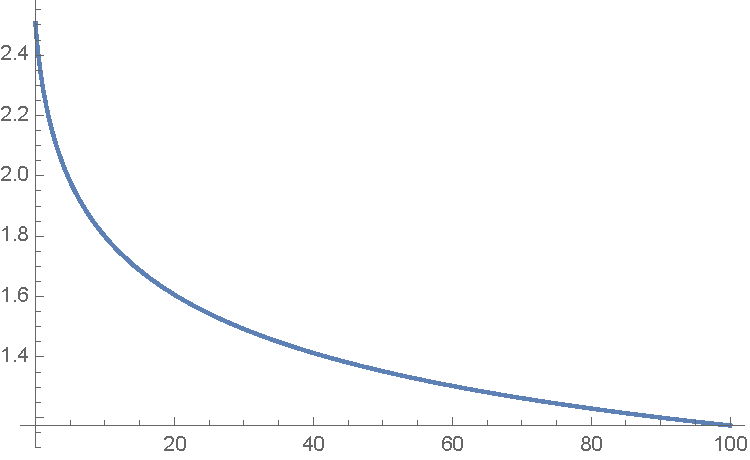
\includegraphics[scale=.8]{figures/partifun.pdf}
    \caption{Plot of $Z$ vs $\lambda$.}
  \end{figure}
The figure \ref{partifun} represents the graph of full function.
\begin{figure}
  \centering
  \label{partifun1}
  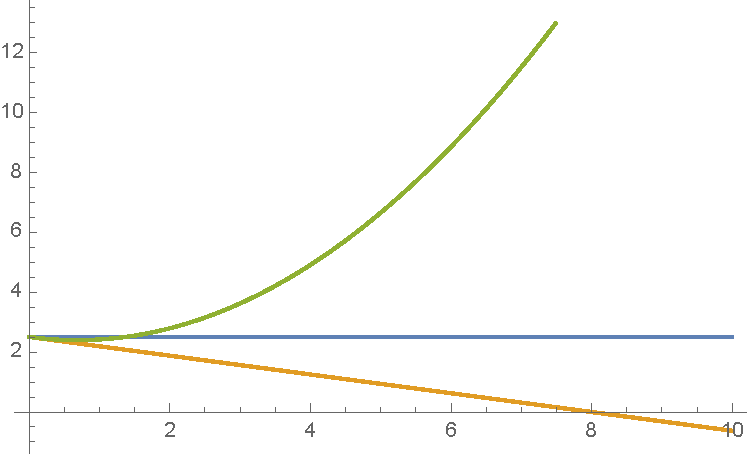
\includegraphics[scale=.8]{figures/partifun1.pdf}
  \caption{Truncated $Z$.}
\end{figure}
Figure \ref{partifun1} represents the truncated $Z$.
\end{solution}

One might wonder whether there could be some \ti{other} series expansion for $Z(m,\lambda)$.
But this is impossible, as the next exercise shows.

\begin{exercise} Do the following:
\begin{enumerate}
\item Show that if $f$ has a convergent Taylor series expansion around $t = 0$ then this expansion
is also an asymptotic expansion as $t \to 0^+$.
\item Show that any $f$ can have at most one asymptotic series expansion.
\end{enumerate}
\end{exercise}


In particular, since $Z(m,\lambda)$ has the divergent asymptotic 
expansion \eqref{eq:0d-perturbation-series} it cannot also
have a convergent one.
For fun, we can diagnose a bit more precisely the problem with $Z$: it has an essential 
singularity at $\lambda = 0$, in the sense of the next exercise.
\begin{exercise} Do the following things.
\begin{enumerate}
\item Show that $Z(m,\lambda) = \frac{1}{\sqrt{m}} f(\tilde\lambda)$ for some $f$.
\item Show that $Z(m,\lambda)$ obeys the differential equation $(2\partial_m)^2 Z = -(4! \partial_\lambda) Z$.
\item Show that $f(\tilde\lambda)$ obeys an ordinary differential equation in $\tilde\lambda$,
with an irregular singularity at $\tilde\lambda = 0$.
\item Show that, for fixed $m$, $Z(m, \lambda)$ admits analytic continuation to a branched cover of $\C \setminus \{ 0 \}$
and this continuation has an essential singularity at $\lambda = 0$.
\item Conclude (again) that $Z(m, \lambda)$ cannot have
a convergent Taylor expansion around $\lambda = 0$.
\end{enumerate}
\end{exercise}

\begin{solution}
  \begin{enumerate}
  \item So the partition function is given by
    \begin{equation}
      \begin{split}
      Z(m,\lambda) &= \int_{-\infty}^{\infty} dx e^{-\left(\frac{1}{2}mx^2+\frac{\lambda}{4!}x^4\right)}\\
      &= \int_{-\infty}^{\infty} dx e^{-\frac{1}{2}mx^2}e^{-\left(1+\frac{2\lambda}{4!m^2}x^2\right)}\\
      &= \left[e^{-\left(1+\frac{2\lambda}{4!}x^2\right)}\int_{-\infty}^{\infty} dx e^{-\frac{1}{2}mx^2}\right]_{-\infty}^{\infty}-\int_{-\infty}^{\infty} dx \frac{d}{dx}e^{-\left(1+\frac{2\lambda}{4!m^2}x^2\right)}\left(\int dx e^{-\frac{1}{2}mx^2}\right)\\
      &= \left(0-\int_{-\infty}^{\infty} dx\sqrt{\frac{\pi}{2m}}\text{erf}\left(\frac{m}{2}x\right) \frac{d}{dx}e^{-\left(1+\frac{2\lambda}{4!m^2}x^2\right)}\right)\\
      &= \frac{1}{\sqrt{m}}f(\tilde{\lambda})
      \end{split}
    \end{equation}
    \item It is very easy to check the identity from the definition $Z(m,\lambda) = \int_{-\infty}^{\infty} dx e^{-\left(\frac{1}{2}mx^2+\frac{\lambda}{4!}x^4\right)}$
    \item Well $Z(m,\lambda)=\frac{1}{\sqrt{m}}f(\tilde{\lambda})$ and from part 2, we have a differential equation.  On combining these two we get
      \begin{equation}
        \begin{split}
          4\partial^2_mZ &= -24\partial_\lambda Z\\
          4\partial^2_m\frac{1}{\sqrt{m}}f(\tilde{\lambda}) &= -24\partial_\lambda \frac{1}{\sqrt{m}}f(\tilde{\lambda})\\
        \end{split}
      \end{equation}
but 
\begin{equation}
  \begin{split}
    \tilde{\lambda} &= \frac{\lambda}{m^2}\\
  \end{split}
\end{equation}
thus
\begin{equation}
        \begin{split}
          3m^{-\frac{5}{2}}f(\tilde{\lambda}) &= -24m^{-2}\partial_{\tilde{\lambda}} \frac{1}{\sqrt{m}}f(\tilde{\lambda})\\
f(\tilde{\lambda}) &= -8\partial_{\tilde{\lambda}}f(\tilde{\lambda})
        \end{split}
      \end{equation}
  \end{enumerate}
\end{solution}

What we have seen here is that even in $0$-dimensional quantum field theory the perturbation series
is ``only'' asymptotic. In higher-dimensional theories, we will meet very similar series, and there
too we expect that these series are usually ``only'' asymptotic.

\begin{exercise} Read the famous paper \cite{Dyson:1952tj} of Freeman Dyson, 
in which he gives a heuristic physical argument that the perturbation series 
in quantum electrodynamics is only asymptotic.
\end{exercise}



\subsection{Feynman diagrams}

Now we revisit \eqref{eq:0d-perturbation-series} and rewrite it one more time, as
\begin{equation} \label{eq:0d-series-rewritten}
  Z(m, \lambda) \, \sim \, \sqrt\frac{2\pi}{m} \sum_{n=0}^\infty \frac{(4n)!}{(2n)! 2^{2n}} \, \frac{(-\tlambda)^n}{(4!)^n n!}, \qquad \tlambda = \frac{\lambda}{m^2}.
\end{equation}
This formula has a neat combinatorial interpretation, in
terms of \ti{Feynman diagrams}, as follows. 

Our basic object is a vertex with $4$ half-edges attached.
% Such a vertex will ``carry'' a factor $-\tlambda$.
\insfig{qft-geometry-1}{0.8}
To construct all Feynman diagrams with $n$ vertices, 
we begin by fixing $n$ vertices, and then considering all ways
to pair up the $4n$ half-edges.
All Feynman diagrams with one vertex, and some with two vertices,
are shown below.
\insfig{qft-geometry-2}{0.9}
Let $D_n$ be the set of all diagrams with $n$ vertices.

\begin{prop}[Counting pairings of $2k$ objects] \label{prop:count-pairings} The number of ways to pair up $2k$ objects, i.e. to divide them into $k$ $2$-element subsets, is $\frac{(2k)!}{k! 2^k}$.
\end{prop}

\begin{exercise} Prove \autoref{prop:count-pairings}.
\end{exercise}

\begin{solution}
  We apply the combinatorial scheme of choosing $2$ elements from $2k$ objects followed by choosing $2$ objects from $2k-2$ objects until we have only $2$ objects left.  Thus the number we are after, is 
  \begin{equation}
    \begin{split}
    N &= \prod_{i=0}^{k-1} {2k-2i\choose 2}\\
    &= \prod_{i=0}^{k-1} {\frac{(2(k-i))!}{(2(k-i-1))!2!}}\\
    &= \frac{(2k)!}{\cancel{(2k-2)!}2!}\frac{\cancel{(2k-2)!}}{(2k-4)!2!}\ldots\frac{2!}{2!}\\
    &= \frac{(2k)!}{2^k}
    \end{split}
  \end{equation}
\color{red}{I have to still explain the $k!$ factor.}
\end{solution}

Thus we have
\begin{equation}
  \abs{D_n} = \frac{(4n)!}{(2n)! 2^{2n}}.
\end{equation}
On the other hand, $D_n$ is naturally acted on by the finite group
\begin{equation}
  G_n = (S_4)^n \rtimes S_n
\end{equation}
(permuting edges attached to a given vertex and also permuting vertices)
which has 
\begin{equation}
 \abs{G_n} = (4!)^n n!. 
\end{equation}
Thus \eqref{eq:0d-series-rewritten} can be rewritten as
\begin{equation}
  Z(m, \lambda) \sim \sqrt\frac{2\pi}{m} \sum_{n=0}^\infty (-\tlambda)^n \frac{\abs{D_n}}{\abs{G_n}}.
\end{equation}
By the orbit-stabilizer theorem this becomes
\begin{equation}
  Z(m, \lambda) \sim \sqrt\frac{2\pi}{m} \sum_{n=0}^\infty (-\tlambda)^n \sum_{[\Gamma] \in D_n / G_n} \frac{1}{\abs{\Aut \Gamma}}
\end{equation}
which we could also rewrite as
\begin{equation}
  Z(m, \lambda) \sim \sqrt\frac{2\pi}{m} \sum_{[\Gamma] \in \sqcup_n D_n / G_n} \frac{(-\lambda)^{\abs{\vertices(\Gamma)}}}{m^{\abs{\edges(\Gamma)}}} \frac{1}{\abs{\Aut \Gamma}}.
\end{equation}
For more information about orbit stablizer theorem, please refer the appendix 

Thus we have proven a diagrammatic rule:

\begin{prop}[Feynman diagram expansion for the partition function \eqref{eq:0d-partition-fn}] \label{prop:0d-feynman} To compute the perturbation
expansion of the partition function \eqref{eq:0d-partition-fn} 
we can follow the following algorithm.
Draw one representative $\Gamma$ in
each equivalence class. Define a weight $w_\Gamma$ as a product of factors: 
one factor $(-\lambda)$ for each vertex,
one factor $\frac{1}{m}$ for each edge,
\insfig{qft-geometry-4}{0.9}
and an overall ``symmetry factor'' $\frac{1}{\abs{\Aut \Gamma}}$.
Then
\begin{equation}
  \frac{Z(m,\lambda)}{Z(m,0)} \sim \sum_\Gamma w_\Gamma.
\end{equation}
\end{prop}
The first few orders in the diagram expansion of $Z(m,\lambda)$ are:
\insfig{qft-geometry-3}{0.8}
This reproduces \eqref{eq:0d-perturbation-series} as it should.

This basic mechanism can be extended in many ways:

\begin{enumerate}
\item In \autoref{prop:0d-feynman} 
we sum over both connected and disconnected $\Gamma$.
But the contribution from disconnected diagrams is easily determined:
\begin{prop}[Exponentiation of the connected diagrams] The sum over connected diagrams is related to the sum over all
diagrams by:
\begin{equation}
  \sum_{\Gamma} w_\Gamma = \exp \left( \sum_{\Gamma \text{ connected nonempty}} w_\Gamma \right).
\end{equation}
\end{prop}
(e.g. look at the first disconnected term above to get an inkling of why.)
Said otherwise,
\begin{equation}
  \log \left( \frac{Z(m,\lambda)}{Z(m,0)} \right) \sim \sum_{\Gamma \text{ connected nonempty}} w_\Gamma.
\end{equation}

\item Suppose we want to compute the correlation function $\IP{x^n}$,
as defined in \eqref{eq:0d-expectation-values} (generalizing $Z$ which is the 
case $n=0$). This is given by a similar sum over Feynman diagrams, except that
now we introduce a new type of $1$-valent vertex, and require that the diagram
contains exactly $n$ of these. The automorphisms of $\Gamma$ are required to
fix these vertices.

To compute the \ti{normalized} expectation value $\IP{x^n} / Z$, we compute
similarly, with the additional rule that every connected component of each diagram
must contain at least one of the $1$-valent vertices.
\insfig{qft-geometry-5}{0.8}

\begin{exercise} Do the following:
\begin{itemize}

\item Compute the perturbative expansion of $\IP{x^2} / Z$ up to order $\lambda^3$, using Feynman diagrams.
You should find $\IP{x^2} / Z = \frac{1}{m} (1 - \frac{1}{2} \tilde\lambda + \frac{2}{3} \tilde\lambda^2 - \frac{11}{8} \tilde\lambda^3 + \cdots )$.
(I drew the diagrams up to order $\tilde\lambda^2$ above.)

\item Compute the perturbative expansion of $\IP{x^4} / Z$ up to order $\lambda^2$, using Feynman diagrams. You should find $\IP{x^4} / Z = \frac{1}{m^2} (3 - 4 \tilde\lambda + \frac{33}{4} \tilde\lambda^2 + \cdots )$.
\end{itemize}
\end{exercise}


\item Instead of the action \eqref{eq:0d-action-quartic} we could take more
generally
\begin{equation}
  S(x) = \frac{m}{2} x^2 + \sum_{k=3}^\infty \frac{\lambda_k}{k!} x^k.
\end{equation}
The Feynman diagram expansion then involves vertices of arbitrary valences,
with each $k$-valent vertex contributing a factor $-\lambda_k$:
\insfig{qft-geometry-6}{0.95}
Here are some diagrams in the expansion of $Z / Z_0$:
\insfig{qft-geometry-7}{0.8}

\item Generalizing in a different direction, we could 
take $\cC = \R^N$ instead of $\R$ (``multiple fields''),
with coordinates $x^1, \dots, x^N$,
and generalize the action to\footnote{Here and in many future equations we are using
the ``Einstein summation convention'': any index which appears both up and down should be 
summed over. So the first term in \eqref{eq:0d-action-multifield} should be read
$\half \sum_{i=1}^N \sum_{j=1}^N x^i M_{ij} x^j$ and similarly the second term involves
four sums.}
\begin{equation} \label{eq:0d-action-multifield}
  S = \half x^i M_{ij} x^j + \frac{1}{4!} C_{ijkl} x^i x^j x^k x^l,
\end{equation}
where $M$ and $C$ are both totally symmetric in their indices.
Then we have
\begin{equation} \label{eq:gaussian-det}
  Z_0 = \int_{\cC} \de \vec{x} \, \e^{-\half x^i M_{ij} x^j} = \frac{(2\pi)^{N/2}}{\sqrt{\det M}}.
\end{equation}
The diagrams $\Gamma$ are just as before, with edges and quartic vertices. However,
in the Feynman rules we attach additional labels $i \in \{1, \dots, N\}$ on the half-edges:
\insfig{qft-geometry-8}{1}
To compute the weight $w_\Gamma$ we sum over all possible labels for
the half-edges (so for a diagram with $k$ edges we sum
$N^{2k}$ terms), and divide by the usual symmetry factor $\abs{\Aut \Gamma}$ 
for the unlabeled diagram $\Gamma$.
(In higher-dimensional QFT, these sorts of labels would have an interpretation
like labeling species of particle which could propagate along the edges.)

A basis-free description of this situation is as follows.
Let $\cC$ be a finite-dimensional real vector space $V$, with a 
translation invariant measure $\de \mu$, and two elements
\begin{equation}
  M \in \Sym^2(V^*), \qquad C \in \Sym^4(V^*).
\end{equation}
Then consider the action
\begin{equation} \label{eq:bosonic-quartic-action}
  S(x) = \half M(x,x) + \frac{1}{4!} C(x,x,x,x).
\end{equation}
$M$ determines a measure $\sqrt{\det M}$ on $V$:
\begin{exercise}
Verify that a bilinear form $M \in \Sym^2(V^*)$ determines a measure on $V$,
which deserves to be called $\sqrt{\det M}$ in the sense that given
a basis $\{e^1, \dots, e^n\}$ on $V$, with $M(e^i,e^j) = M^{ij}$, 
$\sqrt{\det M} = \sqrt{\det (M^{ij})} \abs{e^*_1 \cdots e^*_n}$.
\end{exercise}
When $C = 0$ the partition function is
\begin{equation}
  Z_0 = (2\pi)^{\half \dim V} \frac{\de\mu}{\sqrt{\det M}}.
\end{equation}
The Feynman rules assign a vector in $(V^*)^{\otimes 4}$ to each vertex
and $V^{\otimes 2}$ to each edge, contracted in the obvious way:
\insfig{qft-geometry-14}{0.9}

\end{enumerate}


\subsection{A coupled system}

Now suppose $\cC = \R^2$ and
\begin{equation}
  S(x,y) = \frac{m}{2} x^2 + \frac{M}{2} y^2 + \frac{\mu}{4} x^2 y^2.
\end{equation}
We think of this as two independent systems, one involving the field $x$
and one involving the field $y$, which are ``coupled'' by the quartic interaction
term $\frac{\mu}{4} x^2 y^2$. You can see this point of view vividly in the
Feynman rules for this theory, shown below:
\insfig{qft-geometry-9}{1.0}
\begin{exercise} Explain how these Feynman rules arise as a special case of
the multiple-field rules given above.
\end{exercise}
A few sample computations are:
\insfig{qft-geometry-10}{0.8}

But the job of computing by Feynman diagrams 
in this theory gets complicated fast.
For example:
\insfig{qft-geometry-11}{0.8}
How can we avoid this enormous profusion of diagrams every time we want to 
compute a correlation function?
Suppose that we are only interested in computing correlations involving $x$.
Then to simplify our task, we could use Fubini's theorem to integrate
over $y$ ``once and for all'': define $S_\eff(x)$ by the equation
\begin{equation}
  \int \de y \, \e^{-S(x,y)} = \e^{-S_\eff(x)}
\end{equation}
and then use $S_\eff(x)$ as our action for subsequent computations.

In this particular theory
we can compute the perturbation series of $S_\eff(x)$ explicitly: it is of the form
\begin{equation} \label{eq:seff-series}
  S_\eff(x) \sim \frac{m_\eff}{2} x^2 + \sum_{k \ge 3} \frac{\lambda_k}{k!} x^k
\end{equation}
with
\begin{equation} \label{eq:seff-terms}
  m_\eff = m + \frac{\mu}{2M}, \qquad \lambda_k = \begin{cases} 0 & \text{ for $k$ odd,} \\ - \left( - \frac{\mu}{2M} \right)^{k/2} (k-1)! & \text{ for $k$ even.} \end{cases} 
\end{equation}

Some qualitative remarks about $S_\eff(x)$:
\begin{itemize}
\item Even though the original action $S(x,y)$ had only a quartic interaction, the
effective action $S_\eff(x)$ involves interactions of all even orders.
Diagrammatically speaking, integrating out the field $y$ to pass from $S$ 
to $S_\eff$ amounts to ``collapsing'' parts of the Feynman diagrams
involving only the dashed $y$ lines; these parts get absorbed 
into the new effective vertices.

\item The fact that in the effective theory 
we only get interaction vertices of even valence is
related to the fact that the original action $S(x,y)$ has the symmetry
$x \to -x$, which implies that $S_\eff(x)$ must have the same symmetry.

\item We could approximate $S_\eff(x)$ by the simpler procedure of setting $y=0$ in $S(x,y)$.
This would not give the exact answer, because the fields are coupled: it would
give $m_\eff = m$ and all $\lambda_k = 0$. Thus the shift $m_\eff - m$ and the nonzero 
values of the $\lambda_k$ could be thought of as ``quantum corrections'' which are some vestige
of the field $y$. Note these corrections 
go to zero in the limit $\mu \to 0$ (decoupling) and also go to
zero in the limit $M \to \infty$.
\item The series \eqref{eq:seff-series} for $S_\eff(x)$ actually is convergent, not
only asymptotic.
\end{itemize}

\begin{exercise} Use the effective action $S_\eff(x)$ to compute $\frac{\IP{x^4}}{Z}$ up to order $\mu^2$.
Note that it is a lot easier than using the original action $S(x,y)$, but it indeed agrees
with the result of the computation done above.
\end{exercise}

\begin{exercise} Derive the formula \eqref{eq:seff-terms}.
\end{exercise}

There is also a Feynman-diagram expansion for the computation of the effective action 
$S_\eff$. The rules here
turn out to be as follows: we introduce a new $1$-valent vertex and 
sum over connected diagrams where all $x$ lines are required to terminate on a $1$-valent vertex.
In counting the symmetry factor we do \ti{not} require that these $1$-valent vertices 
are fixed by the automorphisms. The Feynman rules are:
\insfig{qft-geometry-12}{0.95}

\begin{exercise}
Use these Feynman rules to derive \eqref{eq:seff-terms}. (Hint: the first few
diagrams contributing are shown below.)
\end{exercise}
\insfig{qft-geometry-13}{0.8}


\subsection{Symmetries}

Let us return to the original theory with action
\eqref{eq:0d-action-quartic}. In this theory we have
\begin{equation} \label{eq:odd-vanishing}
  \IP{x^n} = 0 \quad \text { for $n$ odd}
\end{equation}
One direct way of seeing this is to make the change
of variables $x \to -x$ in the integral \eqref{eq:0d-partition-fn}.
Since $S(x) = S(-x)$ this change of variables gives
\begin{equation}
  \IP{x^n} = \IP{(-x)^n} = (-1)^n \IP{x^n}
\end{equation}
from which \eqref{eq:odd-vanishing} follows.

The Feynman-diagrammatic expression of \eqref{eq:odd-vanishing}
is that there simply are no possible diagrams with an odd number 
of $1$-valent vertices, since the number of half-edges would then 
be odd, no matter how many $4$-valent vertices we add.
The same wouldn't be true if we allow vertices of odd valence;
of course such vertices arise only when there are
odd-degree terms in $S$, which violate the symmetry $x \to -x$.

More generally, 
\begin{prop}[Symmetries and correlation functions] \label{prop:symmetry-correlators}
Whenever $S: \cC \to \R$ and the measure on $\cC$ are both 
invariant under the action of a group $G$, then we have
\begin{equation} \label{eq:correlator-symmetry}
  \IP{\cO^g} = \IP{\cO}
\end{equation}
where $\cO: \cC \to \R$ is any observable, and $\cO^g = g^* \cO$.
\end{prop}

\begin{exercise} Prove \autoref{prop:symmetry-correlators}.
\end{exercise}

\begin{exercise}
Suppose the space $\Obs$ of all observables $\cO$ is decomposed
into isotypical components, $\Obs = \bigoplus_R \Obs_R$,
where $R$ runs over irreducible representations of $G$.
Show that if $\cO \in \Obs_R$ and $R$ is nontrivial
then $\IP{\cO} = 0$.
\end{exercise}

If $G$ is a Lie group, we can differentiate \eqref{eq:correlator-symmetry} 
to get
\begin{prop}[Infinitesimal symmetries and correlation functions]
Whenever $S: \cC \to \R$ and the measure on $\cC$ are both 
invariant under the action of a Lie group $G$, then we have
\begin{equation}
  \IP{X \cO} = 0
\end{equation}
where $\cO: \cC \to \R$ is any observable, and $X \in \fg$.
\end{prop}

\begin{exercise}
Take $\cC = \R^2$ and $S(x,y) = \half m x^2 + \half m y^2$.
Alternatively, letting $z = x + \I y$, we can say $\cC = \C$
and $S(z) = \half m \abs{z}^2$.
Consider the complex observables $\cO_n: \cC \to \C$ given by
$\cO_n(z) = z^n$.
Use \autoref{prop:symmetry-correlators} to show that the correlation function
$\IP{\cO_n}$ vanishes for all $n \neq 0$. Is the same true if
$S(z) = V(\abs{z})$ for more general $V$? 
What about if $S(z)$ is an arbitrary function of $z$?
\end{exercise}

\subsection{Fermions}

So far, the results of our QFT computations have been very far from
``topological'': $Z$ and all the expectation values
$\IP{x^n}$ are nontrivial functions of the parameters $(m,\lambda)$
with no kind of deformation invariance in sight.

In the applications of QFT toward which we are headed, 
we will do things that are more deformation
invariant. But to get there, we need one more key ingredient: \ti{fermions}.

We will replace the field space $\cC$, which so far has been a manifold
(in fact a vector space), by a \ti{supermanifold} (in fact super vector
space).

Our treatment of supergeometry will be extremely superficial. Some references
I have found useful are \cite{Deligne1999b,etingof,Witten2012,Zakharevich2017}.

\begin{defn}[Super vector space] A \ti{super vector space} is a $\Z/2\Z$-graded vector space,
\begin{equation}
  V = V^0 \oplus V^1.
\end{equation}
\end{defn}

We let $\Pi$ be the operation of \ti{parity reversal}, i.e.
\begin{equation}
  \Pi V = V^1 \oplus V^0.
\end{equation}

\begin{example}The basic example is the super vector space $V$
with $V^0 = \R^p$, $V^1 = \R^q$; call this $\R^{p \vert q}$.
Then $\Pi \R^{p \vert q} = \R^{q \vert p}$.
\end{example}

\begin{defn}[Even and odd maps] An even map of super vector spaces
$V \to W$ is a pair of maps $V^0 \to W^0$ and $V^1 \to W^1$.
An odd map $V \to W$ is a pair of maps $V^0 \to W^1$ and $V^1 \to W^0$.
\end{defn}

\begin{defn}[Category]
A \emph{Category} $C$ consists of 
\begin{enumerate}
\item a class of Obj($C$) objects
\item a class hom($C$) of morphisms between objects
\item there is a composition of morphisms as follows\\
hom($a,b$)$\times$ hom($b,c$) $\to$ hom($a,c$) 
\end{enumerate}
such that the following axioms hold
 \begin{enumerate}
 \item associativity
 \item identity
 \end{enumerate}
\end{defn}

\begin{defn}[Symmetric monoidal category of super vector spaces]
The \ti{symmetric monoidal category} of super vector spaces 
is the category of super vector spaces, with morphisms the even maps,
and equipped with an unusual choice of symmetry isomorphism
\begin{equation}
  s: V \otimes W \to W \otimes V,
\end{equation}
namely, for homogeneous elements $v$, $w$ of degrees $\abs{v}$, $\abs{w}$
we take
\begin{equation}
  s (v \otimes w) = (-1)^{\abs{v} \abs{w}} w \otimes v.
\end{equation}
\end{defn}
This turns out to be a very useful category!

Some standard constructions in linear algebra take on a different
character when applied to super vector spaces. For example,
if $V$ is a super vector space then we define the symmetric 
algebra $\Sym^* V$ to be the quotient of $T^* V$ by
the two-sided ideal generated by $(v \otimes w - s(v \otimes w))$.
If $V = V^0$ then $\Sym^*V$ is (forgetting its super structure) 
the usual $\Sym^* V^0$,
but if $V = V^1$ then $\Sym^* V$ is the exterior algebra $\wedge^* (\Pi V^1)$.

\begin{defn}[Polynomial functions on a super vector space]
Given a super vector space $V$, 
we define the algebra of polynomial functions $\cO(V)$ on $V$
by
\begin{equation}
  \cO(V) = \Sym^* (V^*).
\end{equation}
\end{defn}

$\cO(V)$ is itself a super vector space,
\begin{equation}
  \cO(V) = \cO^0(V) \oplus \cO^1(V),
\end{equation}
and even a (super)commutative algebra.

In quantum field theory we want to consider a space $\cC$ 
with an action $S$ which is some kind of ``function on $\cC$''. 
For $\cC$ a super vector space, our model of ``function on $\cC$''
will be an element
\begin{equation}
S \in \cO^0(V).
\end{equation}


\subsection{A fermionic theory}

The simplest example we can consider is to take
\begin{equation}
  \cC = \R^{0 \vert 2}.
\end{equation}
$\cC$ has two ``coordinate functions''
\begin{equation}
  \psi^1, \psi^2 \in \cO^1(\cC) = (V^1)^*
\end{equation}
but these coordinates have ``odd statistics''
\begin{equation} \label{eq:relations-R02}
  \psi^1 \psi^2 = -\psi^2 \psi^1, \quad (\psi^1)^2 = 0, \quad (\psi^2)^2 = 0.
\end{equation}
Note that $\psi^1 \psi^2 \in \cO^0(\cC)$ is a nice even function,
but \eqref{eq:relations-R02} implies it is nilpotent,
\begin{equation}
  (\psi^1 \psi^2)^2 = 0.
\end{equation}
(In fact $\dim \cO(C) = 2 \vert 2$ as we expect from the identification
with the exterior algebra on $\R^2$; the even part $\cO^0(\cC)$ has basis
$\{1, \psi^1 \psi^2\}$, the odd part $\cO^1(\cC)$ has basis $\{\psi^1, \psi^2\}$.)

Now let us take the action functional
\begin{equation}
  S = \half M \psi^1 \psi^2.
\end{equation}
(Unlike in the bosonic case, here this is all we can do --- there is no 
way of introducing an interaction term!)

We would like to make sense of the partition function in this setting,
\begin{equation} \label{eq:2-fermion-partition-function}
  Z = \int_\cC \de\mu \, \e^{-S}.
\end{equation}
Expanding the exponential, the fact that $S^2 = 0$ means it \ti{truncates} to a polynomial:
\begin{equation} \label{eq:2-fermion-partition-function-expanded}
  Z = \int_\cC \de \mu \, \left(1 - \half M \psi^1 \psi^2\right).
\end{equation}
What will we mean by such an integral?
\ul{Integration over a purely odd vector space is defined to mean taking the
``top order part'' of the function.}
More exactly: 

\begin{defn} \label{defn:odd-integral} A \ti{translation invariant measure} $\de \mu$ 
on a purely odd super vector space $V = V^1$
is
\begin{equation} \label{eq:measure-odd-vector-space}
  \de \mu \in \wedge^\rmtop(\Pi V^1).
\end{equation}
Here top represents the volume form in exterior algebra.
For any $f \in \cO(V) \simeq \wedge^*((\Pi V^1)^*)$, let
$f^\rmtop \in \wedge^\rmtop((\Pi V^1)^*)$ be the top component of $f$; then
we define the integral by
\begin{equation}
  \int_V \de \mu \, f = \de\mu \cdot f^\rmtop.
\end{equation}
\end{defn}

\begin{exercise} Suppose $V = \R^{0 \vert 1}$ with odd coordinate $\psi$.
Show that there exists a translation invariant measure $\de \mu$ on $V$ with the property that
\begin{equation}
\int_V \de \mu \, (a \psi + b) = a.
\end{equation}
We call this measure $\de \psi$.
\end{exercise}

\begin{solution}
  The measure $d\mu\in \wedge^1(\Pi V^1)$ where $V^1=\R^{0|1}$.  We consider the chart $x:\R^{0|1}\to\R$.  In that case, polynomials $f\in\cO(V) \simeq \wedge^1((\Pi V^1)^*)$, are represented by the form $dx$.  We can identify these forms with that of the elements of $\wedge^1(\Pi V^1)$ such that $d\mu:dx\to 1$.  Now the translation invariance $dx(d\mu+c)=dx(d\mu)$ implies $dx(c)=0$ where $c\in\R$.
\end{solution}

\begin{exercise} Again take $V = \R^{0 \vert 1}$, and $c \in \R$.
Show that there exist translation invariant measures $c \de \psi$ and $\de (c \psi)$
on $V$, obeying the formulas
\begin{equation}
  \int_V (c \de \psi) f(\psi) = c \int_V \de \psi f(\psi), \qquad \int_V \de(c \psi) f(c \psi) = \int_V \de \psi f(\psi),
\end{equation}
where $f(c \psi)$ is defined in the obvious way --- explicitly,
if $f(\psi) = a \psi + b$ then $f(c \psi) = a c \psi + b$.
Then prove the change of variables formula in one odd variable:
\begin{equation}
  \de (c \psi) = \frac{1}{c} \de \psi.
\end{equation}
\end{exercise}

\begin{solution}
  
\end{solution}


Similarly on $\R^{0 \vert q}$ we choose once and for all the 
measure $\de \mu = \de \vec\psi$, characterized by
\begin{equation}
  \int \de \vec\psi \, \psi^q \psi^{q-1} \cdots \psi^1 = 1.
\end{equation}
Now we can evaluate the odd Gaussian integral \eqref{eq:2-fermion-partition-function-expanded}, obtaining
\begin{equation} \label{eq:2d-odd-gaussian}
 Z = \half M.  
\end{equation}
Note a key difference between this and the usual even Gaussian integrals:
here the $M$ appears in the \ti{numerator}, not the \ti{denominator}
as we had in \eqref{eq:0d-Z0}.


\subsection{More fermions}

More generally suppose we take $\cC$ to be any 
purely odd super vector space, $\cC = V = V^1$,
equipped with a measure in the sense of \eqref{eq:measure-odd-vector-space},
and elements
\begin{equation}
 M \in \Sym^2(V^*) = \wedge^2((\Pi V^1)^*), \qquad C \in \Sym^4(V^*) = \wedge^4((\Pi V^1)^*).
\end{equation}
Then we can take for the action
\begin{equation}
 S = \half M + \frac{1}{4!} C \in \cO(\cC),
\end{equation}
which we also write in parallel with \eqref{eq:bosonic-quartic-action} as
\begin{equation}
  S(\psi) = \half M(\psi,\psi) + \frac{1}{4!} C(\psi, \psi, \psi, \psi),
\end{equation}
or after choosing a basis for $\Pi V^1$,
\begin{equation}
  S(\psi) = \half M_{IJ} \psi^I \psi^J + \frac{1}{4!} C_{IJKL} \psi^I \psi^J \psi^K \psi^L
\end{equation}
with $M$ and $C$ totally antisymmetric in their indices.

The partition function is an odd integral
\begin{equation}
  Z = \int_\cC \de \mu \, \e^{-S}
\end{equation}
which can again be evaluated in a purely algebraic fashion, by expanding
out the exponential.
\begin{exercise}
Suppose $\cC = \R^{0 \vert 4}$
and $S = m \psi^1 \psi^2 + m \psi^3 \psi^4 + \lambda \psi^1 \psi^2 \psi^3 \psi^4$. Show that $Z = m^2 - \lambda$.
\end{exercise}


\subsection{Perturbation theory}

Integrals over finite-dimensional 
odd vector spaces always give \ti{polynomials} in the couplings; 
thus a development of
``perturbation theory'' for them might seem unnecessary.
Nevertheless, with an eye toward the future, it is interesting to
develop a Feynman diagram expansion for these integrals.

First let us see what happens when $C = 0$.
Then the odd Gaussian integral gives the \ti{Pfaffian} of $M$,
generalizing \eqref{eq:2d-odd-gaussian}
(compare \eqref{eq:gaussian-det}):
\begin{equation} \label{eq:integral-pfaffian}
  Z_0 = \int_\cC \de \vec\psi \, \e^{-\half \psi^I M_{IJ} \psi^J} = \Pf (M).
\end{equation}
(Recall that the Pfaffian is a polynomial in the entries of $M$, defined
only for skew-symmetric $M$, with the property that $(\Pf M)^2 = \det M$.
For example, $\Pf \begin{pmatrix} 0 & a \\ -a & 0 \end{pmatrix} = a$. Note that
for a general $2 \times 2$ matrix the determinant is \ti{not} the square of 
any polynomial.)
\begin{exercise} Prove \eqref{eq:integral-pfaffian}. One way that
presumably works is to expand directly and compare with the
combinatorial expression for the Pfaffian, namely if $\rank M = 2n$ then
\begin{equation}
  \Pf(M) = \frac{1}{2^n n!} \sum_{\sigma \in S_{2n}} (\sgn \sigma) \prod_{i=1}^n M_{\sigma(2i-1), \sigma(2i)}.
\end{equation}
\end{exercise}

When $C \neq 0$ we compute $Z / Z_0$ by Feynman diagrams.
The rules are just as they were in the even case, except that
we have to be careful about signs.
% We fix (arbitrarily) an ordering of the half-edges of the diagram.
% Then, in the contribution from each labeling of the half-edges,
\fixme{...}


\begin{exercise} Suppose again $\cC = \R^{0 \vert 4}$ and $S = m \psi^1 \psi^2 + m \psi^3 \psi^4 + \lambda \psi^1 \psi^2 \psi^3 \psi^4$. Show that $Z = m^2 - \lambda$ by the Feynman diagram expansion. (There is only
one nonempty diagram which contributes.)
\end{exercise}


\subsection{Bosons and fermions together}

Now suppose $\cC = V = V^0 \oplus V^1$ is a super vector space 
which has nontrivial odd \ti{and} even parts. We want to extend
our integration theory to this situation. The strategy will be to 
integrate first over the odd directions, then over 
the even directions.

To get anything convergent,
we need to extend the class of functions we consider:
we let
\begin{equation}
  C^\infty(V) = C^\infty(V^0) \otimes \cO(V^1).
\end{equation}
To define measures we need 
the super analogue of the determinant line:
\begin{defn}[Berezinian line]
The \ti{Berezinian line} of a super vector space $V$ is
\begin{equation}
  \Ber V = \wedge^\rmtop V^0 \otimes \wedge^\rmtop (\Pi V^1)^*.
\end{equation}
\end{defn}
An element $\de \mu \in \Ber V^*$ plays the role of a volume measure
on $V$. By an \ti{orientation} of $V$ we mean an orientation of $V^0$.
Then:
\begin{defn}[Integration over super vector space] If $V$ is an oriented 
super vector space, $\de \mu = \omega^0 \otimes \omega^1 \in \Ber V^*$,
and $f = f^0 \otimes f^1 \in C^\infty(V)$, then
\begin{equation}
    \int_V \de \mu \, f = \int_{V^0} \left( \omega^0 f^0 \right) \int_{V^1} \left( \omega^1 f^1 \right).
\end{equation}
\end{defn}
On $\R^{p \vert q}$ we have the canonical element
\begin{equation}
  \de \mu = \de \vec{x} \, \de \vec{\psi} = (\de x^1 \wedge \cdots \wedge \de x^p) \otimes (\de \vec\psi) \in \Ber V^*.
\end{equation}


\subsection{A supersymmetric example}

Let us now consider the example $\cC = \R^{1 \vert 2}$, and write an action
of the form
\begin{equation} \label{eq:r21-action-generic}
  S(x, \psi^1, \psi^2) = S_1(x) + S_2(x) \psi^1 \psi^2.
\end{equation}
The partition function is
\begin{align}
  Z &= \int \de x \de \vec\psi \, \e^{-S} \\
  &= \int \de x \, S_2(x) \e^{-S_1(x)}.
\end{align}
For generic $S_1(x)$ and $S_2(x)$
we could compute this in perturbation theory:
indeed it just reduces to a computation of the correlation
function $\IP{S_2(x)}$ in 
the pure bosonic theory with action $S_1(x)$.
The answer has no particularly good property.

There is a special case where we can do much better.
(This example is more or less lifted from \cite{MR2003030}.)
This is the case where for some $h: \R \to \R$, with $\abs{h(x)} \to \infty$ 
as $\abs{x} \to \infty$, we have
\begin{equation}
  S_1(x) = \half h(x)^2, \qquad S_2(x) = h'(x),
\end{equation}
so that the action \eqref{eq:r21-action-generic} becomes
\begin{equation}\label{eq:r21-susy-action}
  S(x, \psi^1, \psi^2) = \half h(x)^2 + h'(x) \psi^1 \psi^2.
\end{equation}
The basic reason why this case is better is that the
action \eqref{eq:r21-susy-action} is invariant under a 
certain \ti{odd vector field}
or \ti{supersymmetry}.

\begin{defn}[Graded derivations]
If $\cA$ is a commutative superalgebra, then a map $D: \cA \to \cA$
(either even or odd)
is a \ti{derivation} of $\cA$ if it obeys
\begin{equation}
  D(aa') = (Da)a' + (-1)^{\abs{a} \abs{D}} a(Da').
\end{equation}
\end{defn}

\begin{defn}[Super vector fields on a super vector space]
If $V$ is a super vector space, let $\Vect(V)$ denote the
space of all graded derivations on $C^\infty(V)$.
\end{defn}

In particular, on $\R^{p \vert q}$, in addition
to the usual even vector fields $\partial_{x^i}$ we also have
odd vector fields $\partial_{\psi^I}$, defined by
\begin{equation}
  \partial_{\psi^I} x^i = 0, \quad \partial_{\psi^I} \psi^J = \delta^J_I.
\end{equation}
Together with the derivation property this implies
e.g.
\begin{equation}
  \partial_{\psi^1} \psi^1 \psi^2 = \psi^2, \qquad \partial_{\psi^2} \psi^1 \psi^2 = - \psi^1.
\end{equation}
The $\partial_{x^i}$ and $\partial_{\psi^I}$ together
generate $\Vect(V)$ as a module over $C^\infty(V)$.

\begin{defn}[Super Lie algebra] A \ti{super Lie algebra} is a super
vector space $\fg = \fg^0 \oplus \fg^1$ with a bracket obeying
\begin{equation}
  [X,Y] = -(-1)^{\abs{X} \abs{Y}} [Y,X]
\end{equation}
and
\begin{equation}
[X,[Y,Z]] + (-1)^{\abs{X}(\abs{Y}+\abs{Z})} [Y,[Z,X]] + (-1)^{\abs{Z}(\abs{X}+\abs{Y})}[Z,[X,Y]] = 0.
\end{equation}
\end{defn}

\begin{exercise} Verify that $\Vect(V)$ is 
a super Lie algebra under supercommutator: $[X,Y] f = X(Yf) - (-1)^{\abs{X} \abs{Y}} Y(Xf)$.
\end{exercise}

Now in our example of $\R^{1 \vert 2}$ we consider the
odd vector fields
\begin{align}
  Q_1 &= \psi^1 \partial_x + h(x) \partial_{\psi^2}, \\
  Q_2 &= \psi^2 \partial_x - h(x) \partial_{\psi^1}.
\end{align}
These are both symmetries of the action \eqref{eq:r21-susy-action}, 
in the sense that
\begin{equation}
  Q_1 S = Q_2 S = 0.
\end{equation}

\begin{exercise}
$[Q_1,Q_1]$ is a nontrivial even
vector field on $V$. Compute it, and verify directly 
that it is a symmetry of $S$.
\end{exercise}

The vector fields $Q_1$, $Q_2$ are also divergence-free, i.e. they preserve the
integration measure $\de \mu = \de x \, \de \vec\psi$,
in the following sense.
For any super vector space $F$ we can consider the super vector space
\begin{equation}
  C^\infty(V, F) = C^\infty(V) \otimes_\R F
\end{equation}
which we could think of as a space of ``sections of the trivial super
vector bundle with fiber $F$ over the super vector space $V$.''
Then,

\begin{defn}[Lie derivative of section of $\Ber V^*$ along super vector field] 
If $X$ is a vector field on $V$, the \ti{Lie derivative}\footnote{
For a coordinate-free description of $\cL_X$, more in keeping with
the notion of the infinitesimal variation along a flow which one has in ordinary
geometry, see e.g. \cite{Zakharevich2017}.}
\begin{equation}
  \cL_X: C^\infty(V, \Ber V^*) \to C^\infty(V, \Ber V^*)
\end{equation}
is characterized by
\begin{equation}
 \cL_X (f \de \mu) = (X f) \de \mu + (-1)^{\abs{f} \abs{X}} f \cL_X \de \mu
\end{equation}
and if $X = h^i \partial_{x^i} + g^I \partial_{\psi^I}$ relative to a basis of $V$, then
\begin{equation}
  \cL_{X} ( \de \vec x \, \de \vec\psi ) = \left( \partial_{x^i} h^i + (-1)^{\abs{Q}} \partial_{\psi^I} g^I \right) \de \mu.
\end{equation}
\end{defn}

\begin{exercise} Verify that $\cL_{Q_1} \de \mu = 0$ and similarly
for $Q_2$.
\end{exercise}

The existence of the supersymmetries $Q_1$ and $Q_2$ will give us a 
powerful tool for analyzing the partition function.
First we need a preliminary:

\begin{lem} Suppose $Q$ is a divergence-free vector field
(even or odd)
on a super vector space $V$ with translation invariant measure $\de \mu$, 
and $f \in C^\infty_c(V)$. Then
\begin{equation}
  \int_V \de \mu \, Qf = 0.
\end{equation}
\end{lem}

\begin{pf} By direct computation: if $Q = h^i \partial_{x^i} + g^I \partial_{\psi^I}$ and $\de \mu = \de \vec{x} \de \vec{\psi}$, then
\begin{align}
  \int_V \de \mu \, Qf &= \int \de \vec{x} \, (Qf)^\rmtop \\
  &= \int \de \vec{x} \, (h^i \partial_{x^i} f + g^I \partial_{\psi^I} f)^\rmtop \\
  &= \int \de \vec{x} \, (h^i \partial_{x^i} f + (-1)^{\abs{g}} \partial_{\psi^I} g^I) f)^\rmtop \\
  &= \int \de \vec{x} \, ((- \partial_{x^i} h^i + (-1)^{\abs{g}} \partial_{\psi^I} g^I) f)^\rmtop \\
  &= 0 
\end{align}
where in the second line we used the fact that $(\partial_{\psi^I} (g^I f))^\rmtop = 0$, and in the third line we integrated by parts, 
using the compact support of $f$.
\end{pf}

This permits us to make the following fundamental construction:
\begin{prop}[Invariance of partition function under $Q$-exact deformations] \label{prop:Z-deformation-invariance}
Suppose $V$ is a super vector space with measure $\de \mu$.
Let $\{S_t\}$ be a family of actions,
invariant under a family of divergence-free odd symmetries $Q_t$,
i.e. $Q_t S_t = 0$.
Finally, suppose
\begin{equation}
  \partial_t S_t = Q_t \Psi_t
\end{equation}
with $\Psi_t \in C^\infty_c(\cC)$. 
% , and
% \begin{equation}
%   \IP{ Q_t^2 \Psi_t } = 0
% \end{equation}
% when we compute the expectation value using the action $S_t$.
Then the partition function $Z_t$ computed with action $S_t$
is independent of $t$.
\end{prop}

\begin{pf}
After this deformation the partition function is
\begin{equation}
  Z_t = \int_\cC \de \mu \, \e^{-S_t}
\end{equation}
and thus
\begin{align}
  \partial_t Z_t &= -\int_\cC \de \mu \, (Q_t \Psi_t) \e^{-S_t} \\
  &= -\int_\cC \de \mu \, Q_t \left( \Psi_t \e^{-S_t} \right) \\
  &= 0.
\end{align}
At the first step, to justify the differentiation under the 
integral sign, we use the fact that $\Psi_t$ is compactly supported.
\end{pf}

One often considers the special case where 
$Q_t = Q$ is independent of $t$ and 
has $Q^2 = 0$, in which case it is natural to consider
the \ti{homology} of $Q$ acting on $C^\infty(\cC)$;
in particular $S$ is a $Q$-closed element, and \autoref{prop:Z-deformation-invariance}
says roughly that $Z$ only depends on the \ti{homology class} of $S$.

We will apply \autoref{prop:Z-deformation-invariance} in our example.
We consider deforming the action $S$ in \eqref{eq:r21-susy-action} 
to a family of actions $S_t$, by deforming $h(x)$
to a family $h_t(x)$.
Using dots for derivatives with respect to $t$, we have
\begin{equation}
  \dot S = h(x) {\dot h}(x) + {\dot h}'(x) \psi^1 \psi^2. 
\end{equation}
But this is actually $Q_1$-exact: indeed
\begin{equation} \label{eq:psi-example}
  \dot S = Q_1 \Psi, \qquad \Psi = {\dot h}(x) \psi^2.
\end{equation}
% We do not have $Q_1^2 \Psi = 0$, but the expectation value
% does vanish:
% \begin{exercise}
% Show that $\IP{Q_1^2 \Psi} = 0$.
% \end{exercise}
Thus, applying \autoref{prop:Z-deformation-invariance},
% in this situation, we would conclude that
% $Z$ is completely independent of the function $h(x)$.
% This is actually not true, as we will see momentarily; 
% the reason is that the $\Psi$ appearing in \eqref{eq:psi-example} is not
% compactly supported, spoiling the 
% proof of \autoref{prop:Z-deformation-invariance}.
% Nevertheless:
% \begin{exercise} Show that the differentiation under the
% integral sign in the proof of 
% \autoref{prop:Z-deformation-invariance} is still justified,
% provided that $\deg h_t$ is independent of $t$. 
% \end{exercise}
we conclude:
\begin{prop}[Weak deformation invariance of partition function] 
For the action \eqref{eq:r21-susy-action}, 
$Z$ is unchanged by compactly supported variations of $h$.
\end{prop}

Making deformations with larger and larger compact support $[L,-L]$ and
using an \ti{a priori} estimate of the contribution to $Z$ from
the region $\abs{x} > L$, we can bootstrap to something slightly stronger:
\begin{prop}[Strong deformation invariance of partition function] \label{prop:strong-invariance-0d}
For the action \eqref{eq:r21-susy-action}, 
$Z$ depends only on the asymptotic signs $\eps_+$, $\eps_-$ of $h(x)$,
defined by $\lim_{x \to \pm \infty} h(x) = \eps_{\pm} \infty$.
\end{prop}

\begin{exercise} Prove \autoref{prop:strong-invariance-0d}.
\end{exercise}

As we will see below, one cannot improve this further: $Z$ really
\ti{does} depend on the asymptotic signs $\eps_{\pm}$.
Crudely speaking, the point is that so long as $h(x)^2 \to \infty$
for large $\abs{x}$, it suppresses the contribution to $Z$ 
from large $\abs{x}$, 
making the field space $\cC$ effectively compact. If we try to change
the sign $\eps_+$ (say) by interpolating through a family of functions 
$h_t(x)$, there will be some critical $t$ where we lose this compactness,
and so we lose the deformation invariance.
This is a prototype for ``wall-crossing'' phenomena 
which recur frequently in 
topological QFT. In particular, the failure of Donaldson invariants on $X$
to be fully independent of the metric 
on $X$ when $b_2^+(X) = 1$ has a similar origin.


\subsection{Localization}

We continue with the $0$-dimensional supersymmetric theory of the last section. We want to use the deformation invariance to compute $Z$.

The strategy we follow is roughly to deform $h(x) \to \lambda h(x)$ and take
$\lambda \to \infty$.
In this limit, the bosonic term $h(x)^2$ in the action becomes extremely
large away from the zeroes of $h(x)$; thus one might expect that 
the contribution to $Z$ becomes concentrated near the zeroes,
and can be computed locally there.

Let us recall how the analogous phenomenon plays out for a purely bosonic
integral in one dimension:
consider a family of actions $S_\lambda(x) = \lambda S(x)$,
with all critical points nondegenerate.
Then the $\lambda \to \infty$ asymptotics 
are governed by the method of \ti{steepest descent}.
See \cite{Bender1999} for a very clear account of this method.
\begin{prop}[Steepest descent in one dimension] \label{prop:saddle-expansion-1d-bosonic}
As $\lambda \to \infty$ we have
\begin{equation}
  \int_{-\infty}^\infty \de x \, \e^{-\lambda S(x)} \sim \sum_{x_c: S'(x_c) = 0}
  \sqrt\frac{2 \pi}{\lambda S''(x_c)} \e^{-\lambda S(x_c)}
\end{equation}
\end{prop}
(Of course this expansion is dominated by the critical point(s) where
$S(x_c)$ takes its minimum value: the others are exponentially suppressed,
and could be dropped.)
The proof goes by replacing the original integral by
\begin{equation}
  \sum_{x_c: S'(x_c) = 0} \int_{-\infty}^\infty \de x \, \e^{-\lambda (S(x_c) + \half S''(x_c) (x-x_c)^2)},
\end{equation}
a replacement which (maybe surprisingly) involves only an exponentially small error.

Making the same kind of replacement in our supersymmetric theory leads to
\begin{equation}
  Z(\lambda) \sim \sum_{x_c: h(x_c) = 0} \int \de x \de \vec\psi \, \e^{- \half \lambda h'(x_c)^2 (x-x_c)^2 - \lambda h'(x_c) \psi^1 \psi^2}
\end{equation}
and now performing the Gaussian integrals over fermions and bosons gives
\begin{equation}
  Z(\lambda) \sim \sqrt{2 \pi} \sum_{x_c: h(x_c) = 0} \frac{h'(x_c)}{\abs{h'(x_c)}} = \sqrt{2 \pi} \sum_{x_c: h(x_c) = 0} \sgn(h'(x_c))
\end{equation}
Note the cancellation between the fermions which contribute 
in the numerator and the bosons in the denominator.
Since we already know 
$Z(\lambda)$ is independent of $\lambda$, this proves:
\begin{prop} \label{prop:toy-localization}
In our supersymmetric theory with action \eqref{eq:r21-susy-action},
the partition function can be evaluated exactly:
\begin{equation}
  \frac{Z(\lambda)}{\sqrt{2\pi}} = \sum_{x_c: h(x_c) = 0} \sgn(h'(x_c)) = \half (\eps_+ - \eps_-).
\end{equation}
\end{prop}
\insfig{qft-geometry-15}{0.8}
This is such a toy example that we could have gotten this answer more directly:
\begin{exercise}
Prove \autoref{prop:toy-localization} directly by integrating
out the fermionic directions and then making the formal change of variables
$y = h(x)$.
\end{exercise}

\fixme{study the cancellation in perturbation theory?}

In contrast, expectation values like $\IP{f(x)}$ 
in this theory cannot be evaluated
exactly by localization: the reason is that
functions $f(x)$ are not
$Q$-invariant.


\subsection{Localization in a zero-dimensional sigma model}

Now we consider a less trivial and more geometric example of supersymmetric
localization.
Suppose $(M, \omega)$ is a compact symplectic manifold with
$\dim M = 2n$, with a $U(1)$ action
generated by a Hamiltonian vector field
\begin{equation}
  Y = \omega^{-1}(\de H).
\end{equation}
Suppose moreover that all fixed points of $Y$ are isolated.
Fix some $\alpha \in \R$.
Our interest is in the integral
\begin{equation} \label{eq:dh-integral}
  \int_M \frac{\omega^n}{n!} \e^{\I \alpha H}. 
\end{equation}
\begin{example}
The fundamental example is the case $M = S^2$ with $\omega$ the standard
volume form $\omega = \sin \theta \, \de \theta \wedge \de \varphi$,
and the $U(1)$ action rotating $\varphi$. This action is generated
by the function
\begin{equation}
  H = z = \cos \theta
\end{equation}
and thus
\begin{align}
  \int_M \frac{\omega^n}{n!} \e^{\I \alpha H} &= 2 \pi \int_0^\pi \e^{\I \alpha \cos \theta} \sin \theta \, \de \theta \\
  &= -2 \pi \int_{1}^{-1} \e^{\I \alpha z} \de z \\
  &= \frac{2\pi}{\I \alpha} (\e^{\I \alpha} - \e^{-\I \alpha}) \\
  &= 4 \pi \frac{\sin \alpha}{\alpha}.
\end{align}
\end{example}
This answer exhibits another localization
phenomenon: it is a sum of contributions 
\begin{equation} \label{eq:S2-critical-contrib}
(\pm) \frac{2\pi}{\I \alpha} \e^{\I \alpha H(x_c)}
\end{equation}
from the two fixed points $x_c$ of 
the $U(1)$ action. 

% In short, this is another situation where the
% $\alpha \to \infty$ asymptotic expansion of the integral is 
% unexpectedly also giving the exact answer.

We would like to explain this localization as an instance
of the supersymmetric localization we have been discussing.
For this, we need a generalization of what we have done
so far: we take our field space $\cC$ to be a \ti{supermanifold}
\begin{equation}
 \cC = \Pi T M 
\end{equation}
i.e. the total space of the tangent bundle to $M$,
with the parity of the fibers reversed.
Everything we have done for super vector spaces has
a supermanifold version, obtained by appropriate patching.
I will be vague about this, again referring to the references
\cite{Deligne1999b,etingof,Witten2012,Zakharevich2017} for a
more detailed treatment.

$\cC$ has local charts induced from the charts on $M$.
In each such chart, we identify $\cC$ with a patch of 
$\R^{2n \vert 2n}$, with base coordinates $x^i$ (even)
and fiber coordinates $\psi^i$ (odd). The latter generate an
exterior algebra. Thinking of $\psi^i$ as $\de x^i$, this
suggests that globally we should have
\begin{equation}
  C^\infty(\cC) = \Omega^*(M)
\end{equation}
and this is indeed true.
(More generally, for any $\cC = \Pi E$ with $E \to M$ some vector
bundle we would have $C^\infty(\cC) = C^\infty(M, \wedge^* E^*)$.)

Now we take for our action the function
\begin{equation}
  S = -\I \alpha (H + \omega) = -\I \alpha (H + \omega_{ij} \psi^i \psi^j).
\end{equation}
The partition function is
\begin{equation}
  Z = \int_\cC \de \vec{x} \de \vec{\psi} \, \e^{-S}.
\end{equation}
Here $\de \vec{x} \de \vec{\psi}$ denotes the canonical measure
on $\cC$; this measure exists roughly because the
$\de x^i$ and $\de \psi^i$ transform oppositely under
change of coordinates; more precisely, we have an extension
\begin{equation}
  0 \to \Pi \pi^* TM \to T\cC \to TM \to 0
\end{equation}
from which it follows that $\Ber T\cC = \Ber TM \otimes \Ber \Pi TM$
which is canonically trivial. (The existence of this measure is
the parity-changed analogue of the fact that $T^* M$ has a canonical
volume form.)

Since our supermanifold $\cC$ comes to us as an odd vector bundle, the
rule for integration is a straightforward generalization of what we
have done before: namely we first integrate over the odd directions fiber
by fiber, thus reducing to an integral over the base,
\begin{equation} \label{eq:dh-integrated-over-fibers}
  Z = (\I \alpha)^n \int_M \frac{\omega^n}{n!} \e^{\I \alpha H}.
\end{equation}

\begin{exercise} Verify \eqref{eq:dh-integrated-over-fibers}, by 
computing in a local coordinate patch. (It might be easiest to use 
local Darboux coordinates for $\omega$.)
\end{exercise}

Now we want to compute $Z$ by localization.
Begin by noting that the action $S$ is invariant under the odd vector field
\begin{equation}
  Q = \de + \iota_Y = \psi^i \partial_{x^i} + Y^j \partial_{\psi^j}
\end{equation}
which has (Cartan's formula)
\begin{equation}
  \half [Q,Q] = \cL_Y = \psi^i \partial_{x^i} Y^j \partial_{\psi^j} + Y^i \partial_{x^i}.
\end{equation}
As before, we want to get a localization to some small subset of
$\cC$ by making a perturbation $S \to S + Q \Psi$.
For this we fix a $\U(1)$-invariant metric $g$ on $M$ and then 
take the odd function
\begin{equation}
  \Psi = g(\psi, Y) = g_{ij} \psi^i Y^j = \psi^i Y_i
\end{equation}
where in the last line we defined $Y_i = g_{ij} Y^j$.
Then we have
\begin{equation}
  Q \Psi = g(Y,Y) + \de(gY) = Y^i Y_i - \psi^i \psi^k \partial_{x^k} Y_i
\end{equation}
and 
\begin{equation} \label{eq:Qpsi-closed}
  Q^2 \Psi = 0
\end{equation}
(using the fact that $g$ is $\U(1)$-invariant).
\begin{exercise} Verify \eqref{eq:Qpsi-closed} by direct computation
using the coordinate expressions of $Q$ and $\Psi$.
\end{exercise}

Now we make the deformation $S \to S + \lambda Q \Psi$.
Because of \eqref{eq:Qpsi-closed}, the deformed action is 
still $Q$-invariant, for all values of $\lambda$.
Then, by \autoref{prop:Z-deformation-invariance},
$Z$ is independent of the deformation parameter $\lambda$.
Taking $\lambda$ very large, we can as usual 
reduce to a neighborhood of the zero locus of $g(Y,Y)$, i.e. to the fixed locus of $Y$. Then the steepest-descent method gives
\begin{equation} \label{eq:dh-steepest-descent}
  Z \sim \sum_{x_c \in M: Y(x_c) = 0} \e^{\I \alpha H(x_c)} \times (2\pi)^n \frac{(\de(gY)(x_c))^n/n!}{\sqrt{\det (g(Y,Y))''(x_c)}}
\end{equation}
Here both the numerator
$(\de(gY)(x_c))^n/n!$
and the denominator
$\sqrt{\det (g(Y,Y))''(x_c)}$ 
are valued in $\wedge^\rmtop T^*_{x_c} M$.
\fixme{it would be nicer to be careful about 
twists by orientation bundle here; we always
use the standard orientation to avoid having to worry about it}
What remains is to compute their ratio.

% show that their ratio is
% equal to $(-1)^{n_-} \frac{\omega^n/n!}{\sqrt{\abs{\det H''(x_c)}}}$.
One convenient way to do this is to consider a local model:
$M = \R^2$ with its standard metric and symplectic form,
\begin{equation}
g = \de r^2 + r^2 \de \theta^2, \quad \omega = r \, \de r \wedge \de \theta, 
\end{equation}
with $U(1)$ acting in the charge-$k$ representation,
generated by
\begin{equation}
  Y = k \partial_\theta, \qquad H = \half k r^2.
\end{equation}
Then we compute
\begin{equation}
  \de (gY) = 2 k r \, \de r \wedge \de \theta, \quad \sqrt{\det g(Y,Y)''(0)} = 2 k^2 r \, \de r \wedge \de \theta
\end{equation}
and thus the ratio comes to
\begin{equation}
  \frac{(\de(gY)(x_c))}{\sqrt{\det (g(Y,Y))''(x_c)}} = \frac{1}{k}.
\end{equation}
% while on the other hand
% \begin{equation}
%   \omega = r \de r \wedge \de \theta, \qquad \sqrt{\abs{\det H''(0)}} = \abs{k} r \, \de r \wedge \de \theta
% \end{equation}
% with ratio $1 / \abs{k}$,
% so that the two ratios differ by $\sgn k$.

For an isolated fixed point we can decompose the normal bundle
into a direct sum of $n$ 2-dimensional pieces, with $U(1)$ 
weights $k_1, \dots, k_n$, and put each piece in standard form as
above.
Thus \eqref{eq:dh-steepest-descent} becomes
\begin{equation}
  Z = (2\pi)^n  \sum_{x_c \in M: Y(x_c) = 0} \frac{\e^{\I \alpha H(x_c)}}{\prod_{i=1}^n k_i(x_c)}.
\end{equation}

% The number of negative weights $k_i$ is $\half n_-$.
% Thus finally \eqref{eq:dh-steepest-descent} becomes
% \begin{equation}
%   Z = \sum_{x_c \in M: Y(x_c) = 0} \e^{\I \alpha H(x_c)} \times (2\pi)^n (-1)^{\half n_-} \frac{\e^{\I \alpha H(x_c)} \omega^n}{\sqrt{\abs{\det H''(x_c)}}}
% \end{equation}
Comparing this with \eqref{eq:dh-integrated-over-fibers} proves:

\begin{thm}[Duistermaat-Heckman localization formula \cite{MR674406}] \label{thm:duistermaat-heckman}
\begin{equation} \label{eq:dh-formula}
\int_M \frac{\omega^n}{n!} \e^{\I \alpha H} = \left( \frac{2\pi}{\I \alpha} \right)^{n} \sum_{x_c} \frac{\e^{\I \alpha H(x_c)}}{\prod_{i=1}^n k_i(x_c)}
\end{equation}
where the $k_i(x_c) \in \Z$ are the weights of the $U(1)$ action
on the normal bundle to $x_c$.
\end{thm}

In the case of $S^2$ which we considered above, the weights at the two fixed points
were $k = +1$ and $k = -1$, the sign determined by whether the local orientation induced by the $U(1)$
action agreed or disagreed with the orientation induced by $\omega$.

\begin{exercise} \label{ex:dh-cp2} Work out the concrete 
statement of \autoref{thm:duistermaat-heckman} in the case 
where $M = \C\PP^2$,
with $\omega$ the Fubini-Study \kahler form, 
and the $U(1)$ action given in homogeneous coordinates 
by $(z_1, z_2, z_3) \to (\e^{\I b_1 \theta} z_1, \e^{\I b_2 \theta} z_2, \e^{\I b_3 \theta} z_3)$ for $b_1, b_2, b_3 \in \Z$,
with all $b_i$ distinct.
\end{exercise}

Incidentally,
there is another way of thinking about 
the localization formula \autoref{thm:duistermaat-heckman}. 
The contributions from the fixed points match
what one would get
by making a quadratic approximation to the \ti{original} integrand 
$\omega^n \e^{\I \alpha H}$
around the critical points $x_c$
of $H$. Such an approximation generally gives the leading $\alpha \to \infty$
asymptotics of the integral (this is called the \ti{stationary phase} method,
similar to the steepest descent method which we have been using).
So, \autoref{thm:duistermaat-heckman} can be rephrased
as the statement that, for this particular integral,
 \ti{the stationary phase approximation is exact}.

Since there are a few tricky points here, let us explain 
in a bit more detail how one computes the local contributions 
in the stationary phase method.
A key difference between the stationary phase method and
the steepest-descent expansion is that in the stationary phase 
method we have the
$\I$ in the exponent, hence no exponential suppression. 
One deals with this by rotating the contour of
integration over each real variable by an angle $\pm \pi/4$
into complex space, so that the integrand
becomes exponentially suppressed again.
This produces a factor
\begin{equation}
  \e^{-\frac{\pi \I}{4} (n_+ - n_-)}
\end{equation}
where $(n_+,n_-)$ is the signature of 
the bilinear form $H''(x_c)$.
Then, making the quadratic approximation and performing the Gaussian integral 
leads to the local contribution
\begin{equation}
  \e^{-\frac{\pi \I}{4} (n_+ - n_-)} \left( \frac{2 \pi}{\alpha} \right)^n
\frac{\omega^n/n!}{\sqrt{\abs{\det H''(x_c)}}} \e^{\I \alpha H(x_c)}.
\end{equation}
Looking again at the local models one sees that this is
\begin{equation}
  \e^{-\frac{\pi \I}{4} (n_+ - n_-)} \left( \frac{2 \pi}{\alpha} \right)^n
\frac{\e^{\I \alpha H(x_c)}}{\prod_{i=1}^n \abs{k_i(x_c)}}.
\end{equation}
and since $\half n_-$ is the number of $k_i(x_c)$ which are negative, this
matches the contribution we found in \autoref{thm:duistermaat-heckman}.

I do not really know the significance of the fact that 
the stationary phase
approximation to $\int \omega^n \e^{\I \alpha H}$ 
is exact. As we have seen above, this is \ti{not}
the same method one uses in the supersymmetric localization proof
of \autoref{thm:duistermaat-heckman}, despite the obvious resemblance.

% \begin{thm}[Duistermaat-Heckman localization formula, first version] \label{thm:duistermaat-heckman}
% \begin{equation} \label{eq:dh-formula}
% \int_M \frac{\omega^n}{n!} \e^{\I \alpha H} = \left( \frac{2\pi}{\alpha} \right)^{n} \sum_{x_c} \e^{-\frac{\pi \I}{4} (n_+(x_c) - n_-(x_c))} \frac{\e^{\I \alpha H(x_c)} \omega^n/n!}{\sqrt{\abs{\det H''(x_c)}}}
% \end{equation}
% \end{thm}

\subsection{Some generalizations}

The proof of \autoref{thm:duistermaat-heckman} which we have
given naturally generalizes: we could have replaced the action $S$
by any $Q$-invariant $S \in C^\infty(\cC)$.
Under the identification $C^\infty(\cC) \simeq \Omega^*(M)$,
such an $S$ would be called an \ti{equivariantly closed form}
in the Cartan model for the $U(1)$-equivariant cohomology of $M$,
where $Q$ becomes the \ti{equivariant differential} $\de + \cL_Y$.
Then \autoref{thm:duistermaat-heckman} generalizes to

\begin{thm}[Atiyah-Bott-Berline-Vergne localization for isolated 
fixed points \cite{MR85e:58041,MR705039}] \label{thm:abbv-isolated}
Suppose $M$ is a compact manifold with a $\U(1)$-action, with isolated
fixed points.
Also suppose $\beta \in \Omega^*(M)$ is an equivariantly closed form.
Then
\begin{equation}
\int_M \e^{\beta} = \left( -2\pi \I \right)^{n} \sum_{x_c} \frac{\e^{\beta^\rmbot(x_c)}}{\prod_{i=1}^n k_i(x_c)}
\end{equation}
where $\beta^\rmbot$ means the bottom ($0$-form) component
of $\beta$.
\end{thm}

\begin{exercise} Generalize the proof
of \autoref{thm:duistermaat-heckman} to a proof of \autoref{thm:abbv-isolated}.
\end{exercise}

Finally we can consider a further generalization: let us imagine 
trying to repeat the proof in the case where the fixed points
are not isolated.
In this situation, the leading term in the asymptotics
produced by the steepest-descent method is an integral over the 
fixed locus $F \subset M$.
Thus the supersymmetric localization must reduce $\int_M \e^\beta$
to an integral over $F$. The integrand turns out to be determined by the
local structure around $F$, as follows.

The normal bundle $NF$
has an $\SO(2n)$-structure and connection 
induced by our choice of metric $g$ on $M$,
and a compatible $\U(1)$-action induced by the $\U(1)$-action 
on $M$. \fixme{worry about orientations}

\begin{defn}[Equivariant Euler form] Suppose $X$ is a manifold, with
a $\U(1)$-equivariant $\SO(2n)$-bundle $E$, carrying a 
$\U(1)$-equivariant connection. 
The \ti{equivariant Euler form} of $E$ is \fixme{check signs}
\begin{equation}
  \Euler(E) = \Pf\left(\frac{1}{2\pi} \left(Y + F\right) \right) \in \Omega^*(X)
\end{equation}
where $Y \in \Omega^0(\fso(E))$ is the generator of the $\U(1)$ action
and $F \in \Omega^2(\fso(E))$ is the curvature of the 
equivariant connection on $E$.
\end{defn}
So $\Euler(E)$ is a form concentrated in even degrees.
For example, in the case $n=1$, using the standard trivialization
of $\fso(2)$, we have simply
\begin{equation}
  \Euler(E) = \frac{1}{2\pi} (\I k + F).
\end{equation}
More generally, the bottom component of $\Euler(E)$ is
$\prod_{i=1}^n \frac{\I k_i}{2\pi}$ where the $k_i$ are the weights of the 
$\U(1)$-action. In particular, if no $k_i = 0$ then $\Euler(E)$
has nowhere-vanishing bottom component. This means $\Euler(E)$
is invertible in $\Omega^*(X)$, i.e.
there is a form
\begin{equation}
  \frac{1}{\Euler(E)} \in \Omega^*(X).
\end{equation}

\begin{exercise}
Write the form $\frac{1}{\Euler(E)}$ explicitly in the case $n=1$.
\end{exercise}

% defined using the series expansion
% \begin{equation}
%   \frac{1}{c + x} = \frac{1}{c} (1 - c^{-1} x + c^{-2} x^2 + \cdots)
% \end{equation}
% which is finite when $x$ is nilpotent.
We use this in the statement of the next theorem:

\begin{thm}[Atiyah-Bott-Berline-Vergne localization in general \cite{MR85e:58041,MR705039}] \label{thm:abbv}
Suppose $M$ is a compact manifold with a $\U(1)$-action, with fixed locus
$F$.
Also suppose $\beta \in \Omega^*(M)$ is an equivariantly closed form.
Choose a $\U(1)$-invariant metric $g$ on $M$. Then
\begin{equation}
\int_M \e^{\beta} = \int_F \frac{\e^{\beta}}{\Euler(NF)}.
\end{equation}
\end{thm}

\begin{exercise} Show that \autoref{thm:abbv} reduces to
\autoref{thm:abbv-isolated} when the fixed points of the
$\U(1)$-action are isolated.
\end{exercise}

\begin{exercise} Use \autoref{thm:abbv} to generalize
\autoref{ex:dh-cp2} to the case
where the $b_i$ need not be distinct.
\end{exercise}

\begin{exercise} Generalize the proof
of \autoref{thm:abbv-isolated} to a proof of \autoref{thm:abbv}. \fixme{hard? at least needs more delicacy with the steepest descent expansion}
\end{exercise}


\section{QFT in \texorpdfstring{$1$}{1} dimension}

Now we move to $1$-dimensional quantum field theory.
So we will introduce a Riemannian $1$-manifold $(X,\eta)$ (``spacetime'').
$X$ will be one of
\begin{equation}
  X = \R, \quad X = I, \quad X = S^1.
\end{equation}
We often parameterize $X$ by $t$ which we sometimes
think of as the ``time.''

Our configuration space $\cC_X$ will now be some kind of space
of ``functions on $X$.''


\subsection{The \texorpdfstring{$1$}{1}-dimensional sigma model}

Fix the data:
\begin{itemize}
  \item A Riemannian manifold $(Y,g)$,
  \item A function $V: Y \to R$ (``potential'').
\end{itemize}

We take our field space to be \fixme{be sharper about this}
\begin{equation}
  \cC_X = \Map(X,Y),
\end{equation}
and our action
\begin{align}
  S(\phi) &= \int_X \dvol_X \left(\half g(\dot\phi,\dot\phi) + V(\phi)\right) \\
  &= \int_X \de t \sqrt{\eta_{tt}} \left(\half g_{ij}(\phi) \dot\phi^i \dot\phi^j \eta^{tt} + V(\phi)\right).
\end{align}
If we choose the parameter $t$ on $X$ to be the arc-length, then
this reduces to
\begin{equation}
    S(\phi) = \int_X \de t \, \left( \half g_{ij}(\phi) \dot\phi^i \dot\phi^j + V(\phi) \right).
\end{equation}
This $1$-dimensional quantum field theory is equivalent to
the usual model of nonrelativistic \ti{quantum mechanics},
describing a single particle propagating on $Y$.
Then we can think of the various $\phi \in \cC_X$ as various possible
trajectories that the particle could take.

Now \ti{formally} we would like to consider the partition function,
\begin{equation}
  Z_{S^1} = \int_{\cC_{S^1}} \de \phi \, \e^{-S}
\end{equation}
or the analogue on the interval $I = [0,T]$,
\begin{equation} \label{eq:1d-Z-interval}
  Z_{[0,T]}(y_0, y_1) = \int_{\cC_{[0,T]}(y_0,y_1)} \de \phi \, \e^{-S}
\end{equation}
where we defined
\begin{equation}
  \cC_{[0,T]}(y_0, y_1) = \{\phi: [0,T] \to Y \, \vert \, \phi(0) = y_0, \phi(T) = y_1\}.
\end{equation}
Thus we can view \eqref{eq:1d-Z-interval} 
as a sum over all possible paths
a particle can take from $y_0$ to $y_1$.
\insfig{qft-geometry-16}{0.8}

\appendix

\section{Background}

Here I collect a little background material for convenience; I will probably
not lecture on this material.

\subsection{Spinors}

Good references for this are \cite{MR1031992,MR1367507}.

\begin{defn}[Free graded tensor algebra] Fix a real vector space $V$. The
\ti{free graded tensor algebra} $T(V)$ is
\begin{equation}
  T(V) = \bigoplus_{n=0}^\infty V^{\otimes n}
\end{equation}
equipped with the concatenation product
\begin{equation}
  (v_1 \otimes \cdots \otimes v_n) (w_1 \otimes \cdots \otimes w_m) = v_1 \otimes \cdots \otimes v_n \otimes w_1 \otimes \cdots \otimes w_m
\end{equation}
and the obvious $\Z$-grading.
\end{defn}

\begin{defn}[Clifford algebra] Fix a real vector space $V$ with a positive definite
quadratic form $\IP{\cdot,\cdot}$. The \ti{Clifford algebra} $\Cliff(V)$ is the quotient
of $T(V)$ by the two-sided ideal generated by the relation
\begin{equation} \label{eq:clifford-relation}
  v \otimes v = -\IP{v,v}, \qquad v \in V.
\end{equation}
\end{defn}
More informally we could say $\Cliff(V)$ is the free algebra on $V$
subject to the single relation \eqref{eq:clifford-relation}.
This relation violates the $\Z$-grading but preserves a residual $\Z/2\Z$.
Thus $\Cliff(V)$ is a $\Z/2\Z$-graded algebra:
\begin{equation}
  \Cliff(V) = \Cliff^+(V) \oplus \Cliff^-(V).
\end{equation}

% In \eqref{eq:clifford-relation} we introduced a notation which we will use
% many times in the rest of the course: in graded algebras we have the
% graded commutator, defined on homogeneous elements by the formula
% \begin{equation}
%   [a, b] = ab - (-1)^{\deg a} (-1)^{\deg b} ba.
% \end{equation}

If we allow $\IP{\cdot,\cdot}$ to be the zero quadratic form then $\Cliff(V)$
becomes the exterior algebra $\wedge^*(V)$; more generally $\Cliff(V)$ is
a \ti{deformation} of $\wedge^*(V)$, or, it is a $\Z$-\ti{filtered} algebra 
whose associated $\Z$-graded algebra is $\wedge^*(V)$.

\begin{exercise} Show that $\dim_\R \Cliff(V) = 2^{\dim V}$.
\end{exercise}

\begin{defn}[Pin group] $\Pin(V)$ is the group of all elements
\begin{equation}
 v_1 \otimes v_2 \otimes \cdots \otimes v_n \in \Cliff(V)
\end{equation}
where all $v_i$ have $\norm{v_i}^2 = 1$.
\end{defn}

\begin{defn}[Spin group] $\Spin(V) = \Pin(V) \cap \Cliff^+(V)$.
\end{defn}

As a convenient notation we let $\Cliff(n)$ mean the Clifford algebra on the
vector space $\R^n$ with its standard positive definite quadratic form,
and similarly $\Spin(n)$, $\Pin(n)$ etc.

\begin{exercise} Show that:
\begin{itemize}
\item $\Cliff(1) \simeq \C$, $\Cliff^+(1) \simeq \R$, $\Spin(1) \simeq \Z / 2\Z$.
\item $\Cliff(2) \simeq \bbH$, $\Cliff^+(2) \simeq \C$, $\Spin(2) \simeq \U(1)$.
\item $\Cliff(3) \simeq \bbH \oplus \bbH$, $\Cliff^+(3) \simeq \bbH$, $\Spin(3) \simeq \SU(2)$.
\end{itemize}
\end{exercise}

\begin{prop}[Spin group double-covers $\SO$ group] When $\dim V \ge 2$ 
there is a canonical double-covering map
\begin{equation}
  \Spin(V) \to \SO(V).
\end{equation}
\end{prop}

When $n > 2$, $\Spin(n)$ is simply connected, so this map identifies
$\Spin(n)$ as the universal covering of $\SO(n)$.

\begin{defn}[Spin structures] Fix an oriented manifold $X$, and let $P$ be its principal $\SO(n)$-bundle
of oriented frames. A \ti{spin structure on $X$} is a lift of $P$ to a $\Spin(n)$-bundle.
\end{defn}

\begin{defn}[$\Spin^c$ structures] \fixme{...}
\end{defn}

\begin{prop}[Spin representations] If $n$ is odd, $\Spin(n)$ admits a unique
irreducible complex representation (up to equivalence) with the property that it 
extends to a representation of $\Cliff(n)$; call this representation $S$; it has
$\dim_\C S = 2^{k}$ where $n = 2k+1$.
If $n$ is even, then $\Spin(n)$ admits two such representations (up to equivalence); call them $S^\pm$;
both have $\dim_\C S^{\pm} = 2^k$ where $n = 2k$.
\end{prop}

\begin{defn}[Spinor bundles] \fixme{...}
\end{defn}

\begin{defn}[Dirac operator] \fixme{...}
\end{defn}

\subsection{Hodge theory}

\begin{defn}[Formal adjoint of $\de$]
If $X$ is a Riemannian manifold of dimension $n$,
the formal adjoint of $\de$
is the operator
\begin{equation}
  \de^*: \Omega^{k}(X) \to \Omega^{k-1}(X)
\end{equation}
given by
\begin{equation}
  \de^* = (-1)^{n(k+1)+1} \star \de \star.
\end{equation}
\end{defn}

If $X$ is a compact Riemannian manifold, we have
the $L^2$ pairing on $\Omega^*(X)$ given by
\begin{equation}
  \IP{\alpha,\beta} = \int_X \IP{\alpha(x),\beta(x)} \, \de vol_X = \int_X \alpha \wedge \star \beta.
\end{equation}

\begin{lem}[Formal adjoint is actual adjoint on compact manifold]
If $X$ is a compact Riemannian manifold, $\de^*$ is the actual adjoint
with respect to the $L^2$ pairing, i.e.
\begin{equation}
  \IP{\de^* \alpha,\beta} = \IP{\alpha,\de \beta}.
\end{equation}
\end{lem}

\begin{defn}[Laplace operator on Riemannian manifold]
If $X$ is a Riemannian manifold, we define the form Laplacian
\begin{equation}
  \Delta: \Omega^k(X) \to \Omega^k(X)
\end{equation}
by
\begin{equation} \label{eq:form-laplacian}
  \Delta = \de \de^* + \de^* \de.
\end{equation}
\end{defn}
\fixme{...}

<<<<<<< HEAD
\subsection{Orbit-stablizer theorem}
Let $G$ be a group acting on the finite set $X$. 
\begin{defn}
  The orbit Orb($x$) of an element $x\in X$ is defined as defined as 
  \begin{equation}
    \text{Orb}(x):={y\in X:g\in G:y=g*x}
  \end{equation}
where $*$ denotes the group action of $G$ on the set $X$
\end{defn}
=======

\subsection{Symplectic manifolds}

\begin{defn}[Nondegenerate skew pairing] \label{def:nondegenerate-skew-pairing}
Suppose $V$ is a vector space over $\R$ or $\C$.
We say $\omega \in \wedge^2(V)$ is \ti{nondegenerate}
if the map
\begin{align}
  V &\to V^* \\
  v &\mapsto \iota_v \omega = \omega(v,\cdot)
\end{align}
is an isomorphism.
\end{defn}

\begin{prop}[Standard basis for a nondegenerate skew pairing]
\label{prop:standard-nondegenerate-skew-pairing}
If $V$ is a finite-dimensional vector space over $\R$ or $\C$, and
$\omega \in \wedge^2(V)$ is nondegenerate, then $V$ has
dimension $2n$ for some $n$, and there
exists a basis $\{e_1, \dots, e_n, f_1, \dots, f_n\}$ for $V$
such that
\begin{align}
\omega(e_i, f_j) &= \delta_{ij}, \\
\omega(e_i, e_j) &= 0, \\
\omega(f_i, f_j) &= 0.
\end{align}
\end{prop}

\begin{defn}[Symplectic manifold] \label{def:symplectic-manifold}
A \ti{symplectic manifold} is a pair $(X,\omega)$
where $X$ is a manifold and
$\omega \in \Omega^2(X)$, such that
\begin{equation}
  \de \omega = 0
\end{equation}
and $\omega(x)$ is nondegenerate for every $x \in X$.
\end{defn}

\begin{defn}[Exact symplectic manifold]
An \ti{exact symplectic manifold} is a tuple $(X,\omega,\lambda)$
where $(X,\omega)$ is a symplectic manifold and $\lambda \in \Omega^1(X)$ has $\de \lambda = \omega$.
\end{defn}

\begin{example}[Cotangent bundle is an exact symplectic manifold]
If $X$ is any manifold and $Y = T^* X$, then $Y$ carries a canonical
$1$-form (``Liouville form''), $\lambda \in \Omega^1(Y)$,
defined as follows:
\begin{equation}
  \lambda(x,p) \cdot v = p \cdot \pi_* v \qquad x \in X, p \in T^*_x X, v \in TY.
\end{equation}
Then there is a canonical symplectic form on $Y$ given by
\begin{equation}
\omega = \de \lambda.
\end{equation}
\end{example}

\begin{exercise}
Show that, in the canonical coordinate system $(p_i,q_i)$
on $T^* X$ induced by a coordinate system $(q_i)$ on $X$,
we have
$\lambda = \sum_{i=1}^n p_i \de q_i$, and
$\omega = \sum_{i=1}^n \de p_i \wedge \de q_i$.
\end{exercise}


\begin{defn}[Moment map] \label{def:moment-map}
Suppose $X$ is a symplectic manifold, with symplectic form $\omega$,
acted on by a real Lie group $G$. Let $\fg = \Lie G$ and let
\begin{equation}
\rho: \fg \to \Vect(X)
\end{equation}
be the infinitesimal action.
Suppose given a function
\begin{equation} \label{eq:moment-map}
 \mu: X \to \fg^*
\end{equation}
and for $Z \in \fg$ write $\mu_Z = \mu \cdot Z$.
We say $\mu$ is a \ti{moment map} for the $G$-action if
for all $Z \in \fg$ we have
\begin{equation} \label{eq:moment-map-condition-3}
  \iota_{\rho(Z)} \omega = \de \mu_Z,
\end{equation}
and in addition the map \eqref{eq:moment-map} is $G$-equivariant
(for the $G$-action on $X$ and the coadjoint $G$-action on $\fg^*$).
\end{defn}
In particular, the moment map $\mu$
\ti{determines} the $G$-action.

Note that moment maps do not always exist.
At the very least, the existence of a moment
map requires that $\iota_{\rho(Z)} \omega$ is closed
for all $Z \in \fg$, by \eqref{eq:moment-map-condition-3}. Using
Cartan's ``magic formula''
\begin{equation} \label{eq:cartan-magic-formula}
  \cL_v \omega = \de (\iota_v \omega) + \iota_v (\de \omega)
\end{equation}
and the fact that $\de \omega = 0$,
this is equivalent to requiring $\cL_{\rho(Z)}\omega = 0$,
i.e. the $G$-action preserves $\omega$ infinitesimally.
But even if the $G$-action preserves $\omega$,
a moment map still may not exist.\footnote{When $G$ is compact,
moment maps exist at least
\ti{locally} on $X$, though maybe not globally. When $G$ is not
compact there can even be a local obstruction.}

Conversely, if a moment map $\mu$ does exist and $\fg$
has nontrivial center, we can get another moment map by taking
$\mu' = \mu + c$, where $c$ is fixed by the \ti{coadjoint}
action of $G$, i.e. $c \in [\fg,\fg]^\perp \subset \fg^*$.

\begin{exercise}
Suppose $X = \R^2$ with $\omega = \de x_1 \wedge \de x_2$, and
$G = SO(2) = U(1) = \{e^{\I \alpha}: \alpha \in \R \}$.
Then $\fu(1)$ is $1$-dimensional, spanned by $\partial_\alpha$.
Show that the counterclockwise rotation action of $U(1)$ on $X$,
given by the matrices
\begin{equation}
   \begin{pmatrix} \cos \alpha & - \sin \alpha \\ \sin \alpha & \cos \alpha \end{pmatrix},
 \end{equation}
has a moment map $\mu: \R^2 \to \fu(1)^*$, given by
\begin{equation}
  \mu(x_1,x_2) \cdot \partial_\alpha = -\half (x_1^2 + x_2^2).
\end{equation}
\end{exercise}
Thus if we identify $\fu(1) \simeq \R$ using the generator
$\partial_\alpha$, we can think of $\mu$ just as an $\R$-valued function
on $X$,
\begin{equation}
  \mu(x_1,x_2) = -\half (x_1^2 + x_2^2).
\end{equation}

\begin{exercise} \label{exc:cotangent-moment-map}
Suppose $X$ is any manifold, with a compact
group $G$ acting. Then $T^* X$ is a symplectic manifold
which also has a canonical action of $G$. Verify that
\begin{equation}
  \mu_Z(x,p) = -p \cdot (\rho(Z)(x)) \qquad x \in X, p \in T^*_x X
\end{equation}
gives a moment map for this action.
\end{exercise}

>>>>>>> upstream/master

\printbibliography




\end{document}